\chapter{Атлас облаков}\label{app:5}

  \begin{sidewaysfigure*}
    \centering
    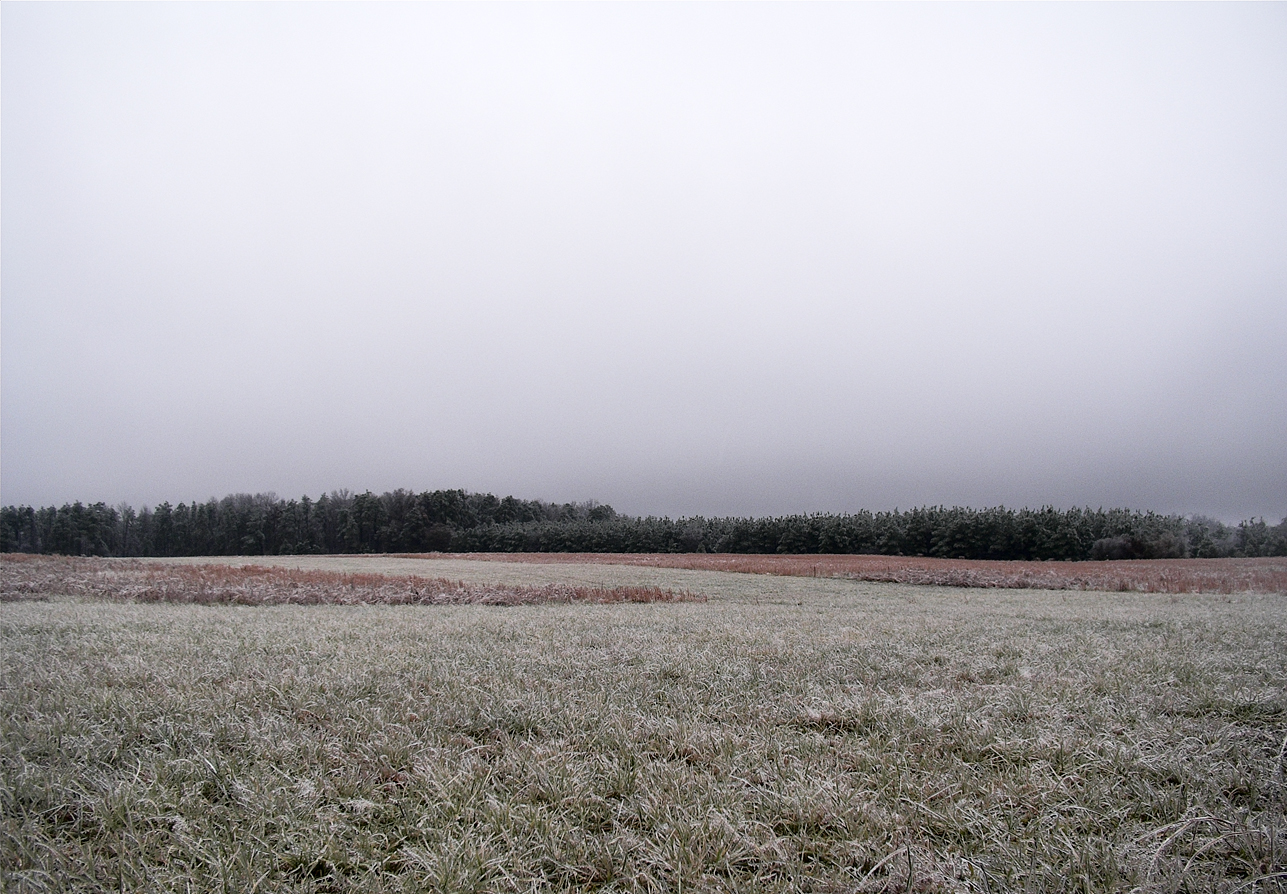
\includegraphics[width=0.9\textheight,keepaspectratio=true]{clouds/stratus_opacus_uniformis}
    \caption[Stratus opacus uniformis]{Stratus opacus uniformis\protect}
    \label{fig:stratus}
    % https://commons.wikimedia.org/wiki/File:Stratus-Opacus-Uniformis.jpg
  \end{sidewaysfigure*}

  \begin{sidewaysfigure*}
    \centering
    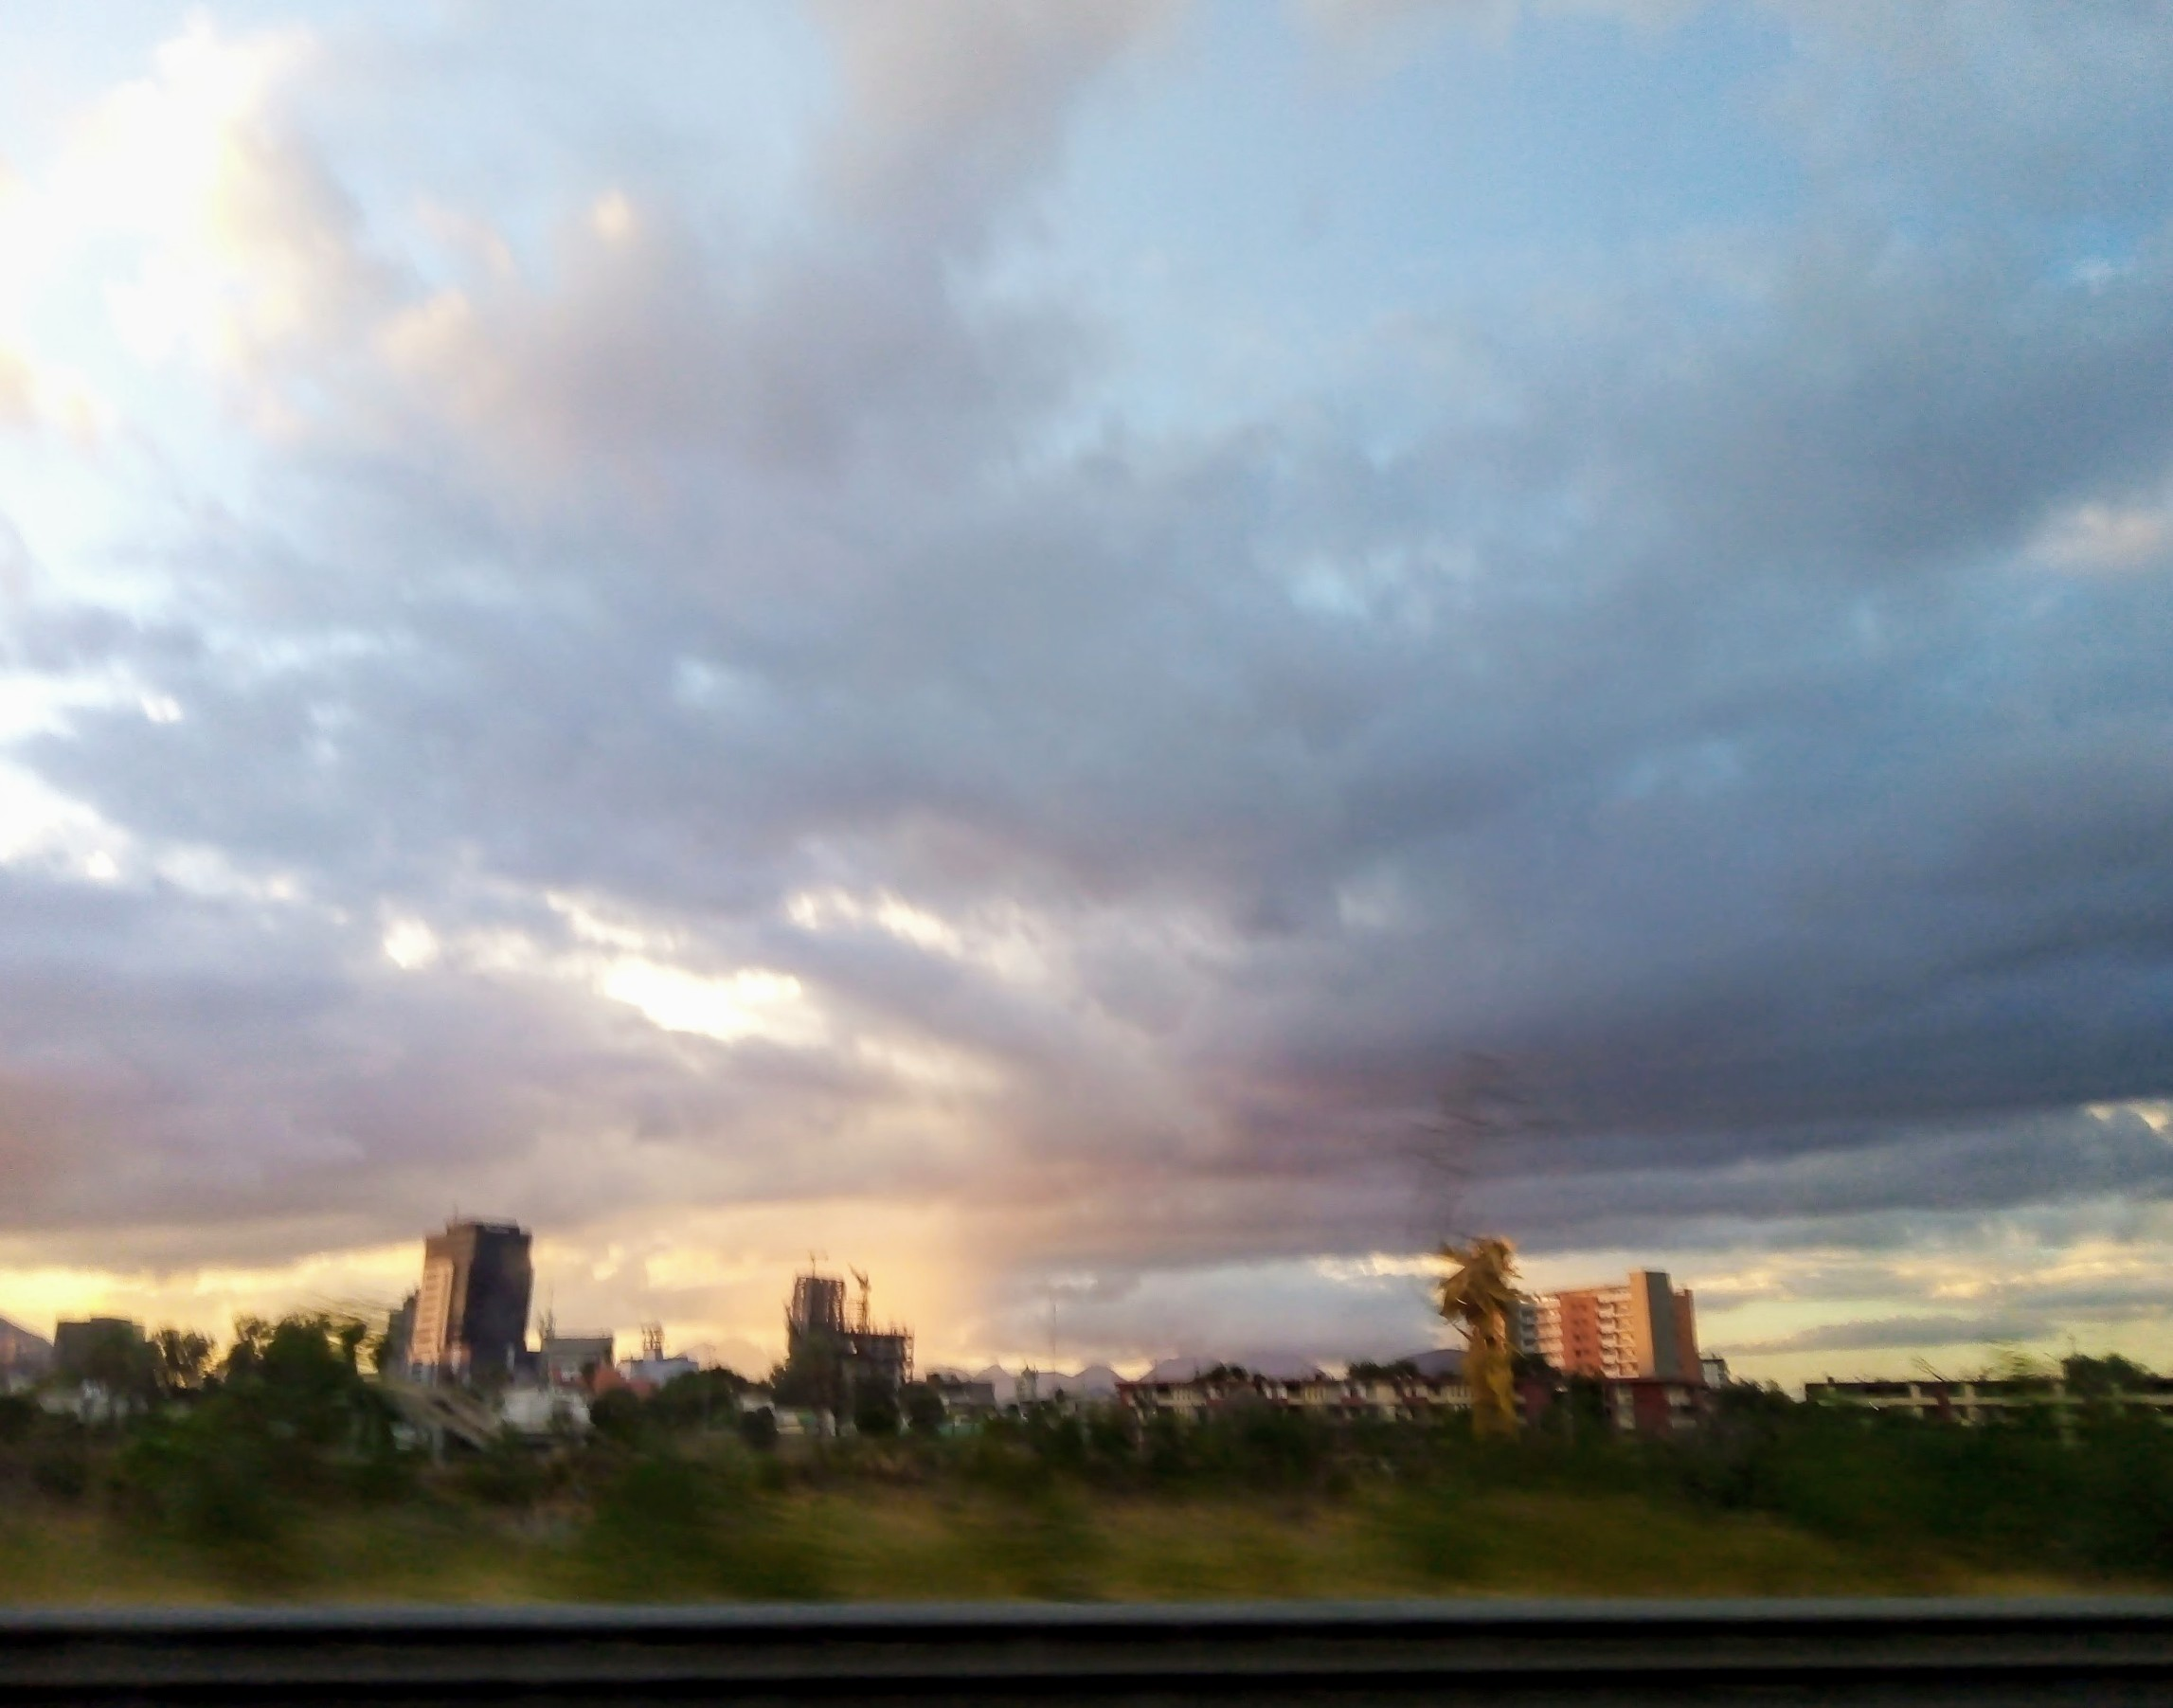
\includegraphics[width=0.9\textheight,keepaspectratio=true]{clouds/stratocumulus_opacus}
    \caption{Stratocumulus opacus}
    \label{fig:stratocumulus-opacus}
    % https://commons.wikimedia.org/wiki/File:Stratocumulus_stratiformis_opacus_praecipitatio_1.jpg
  \end{sidewaysfigure*}

  \begin{sidewaysfigure*}
    \centering
    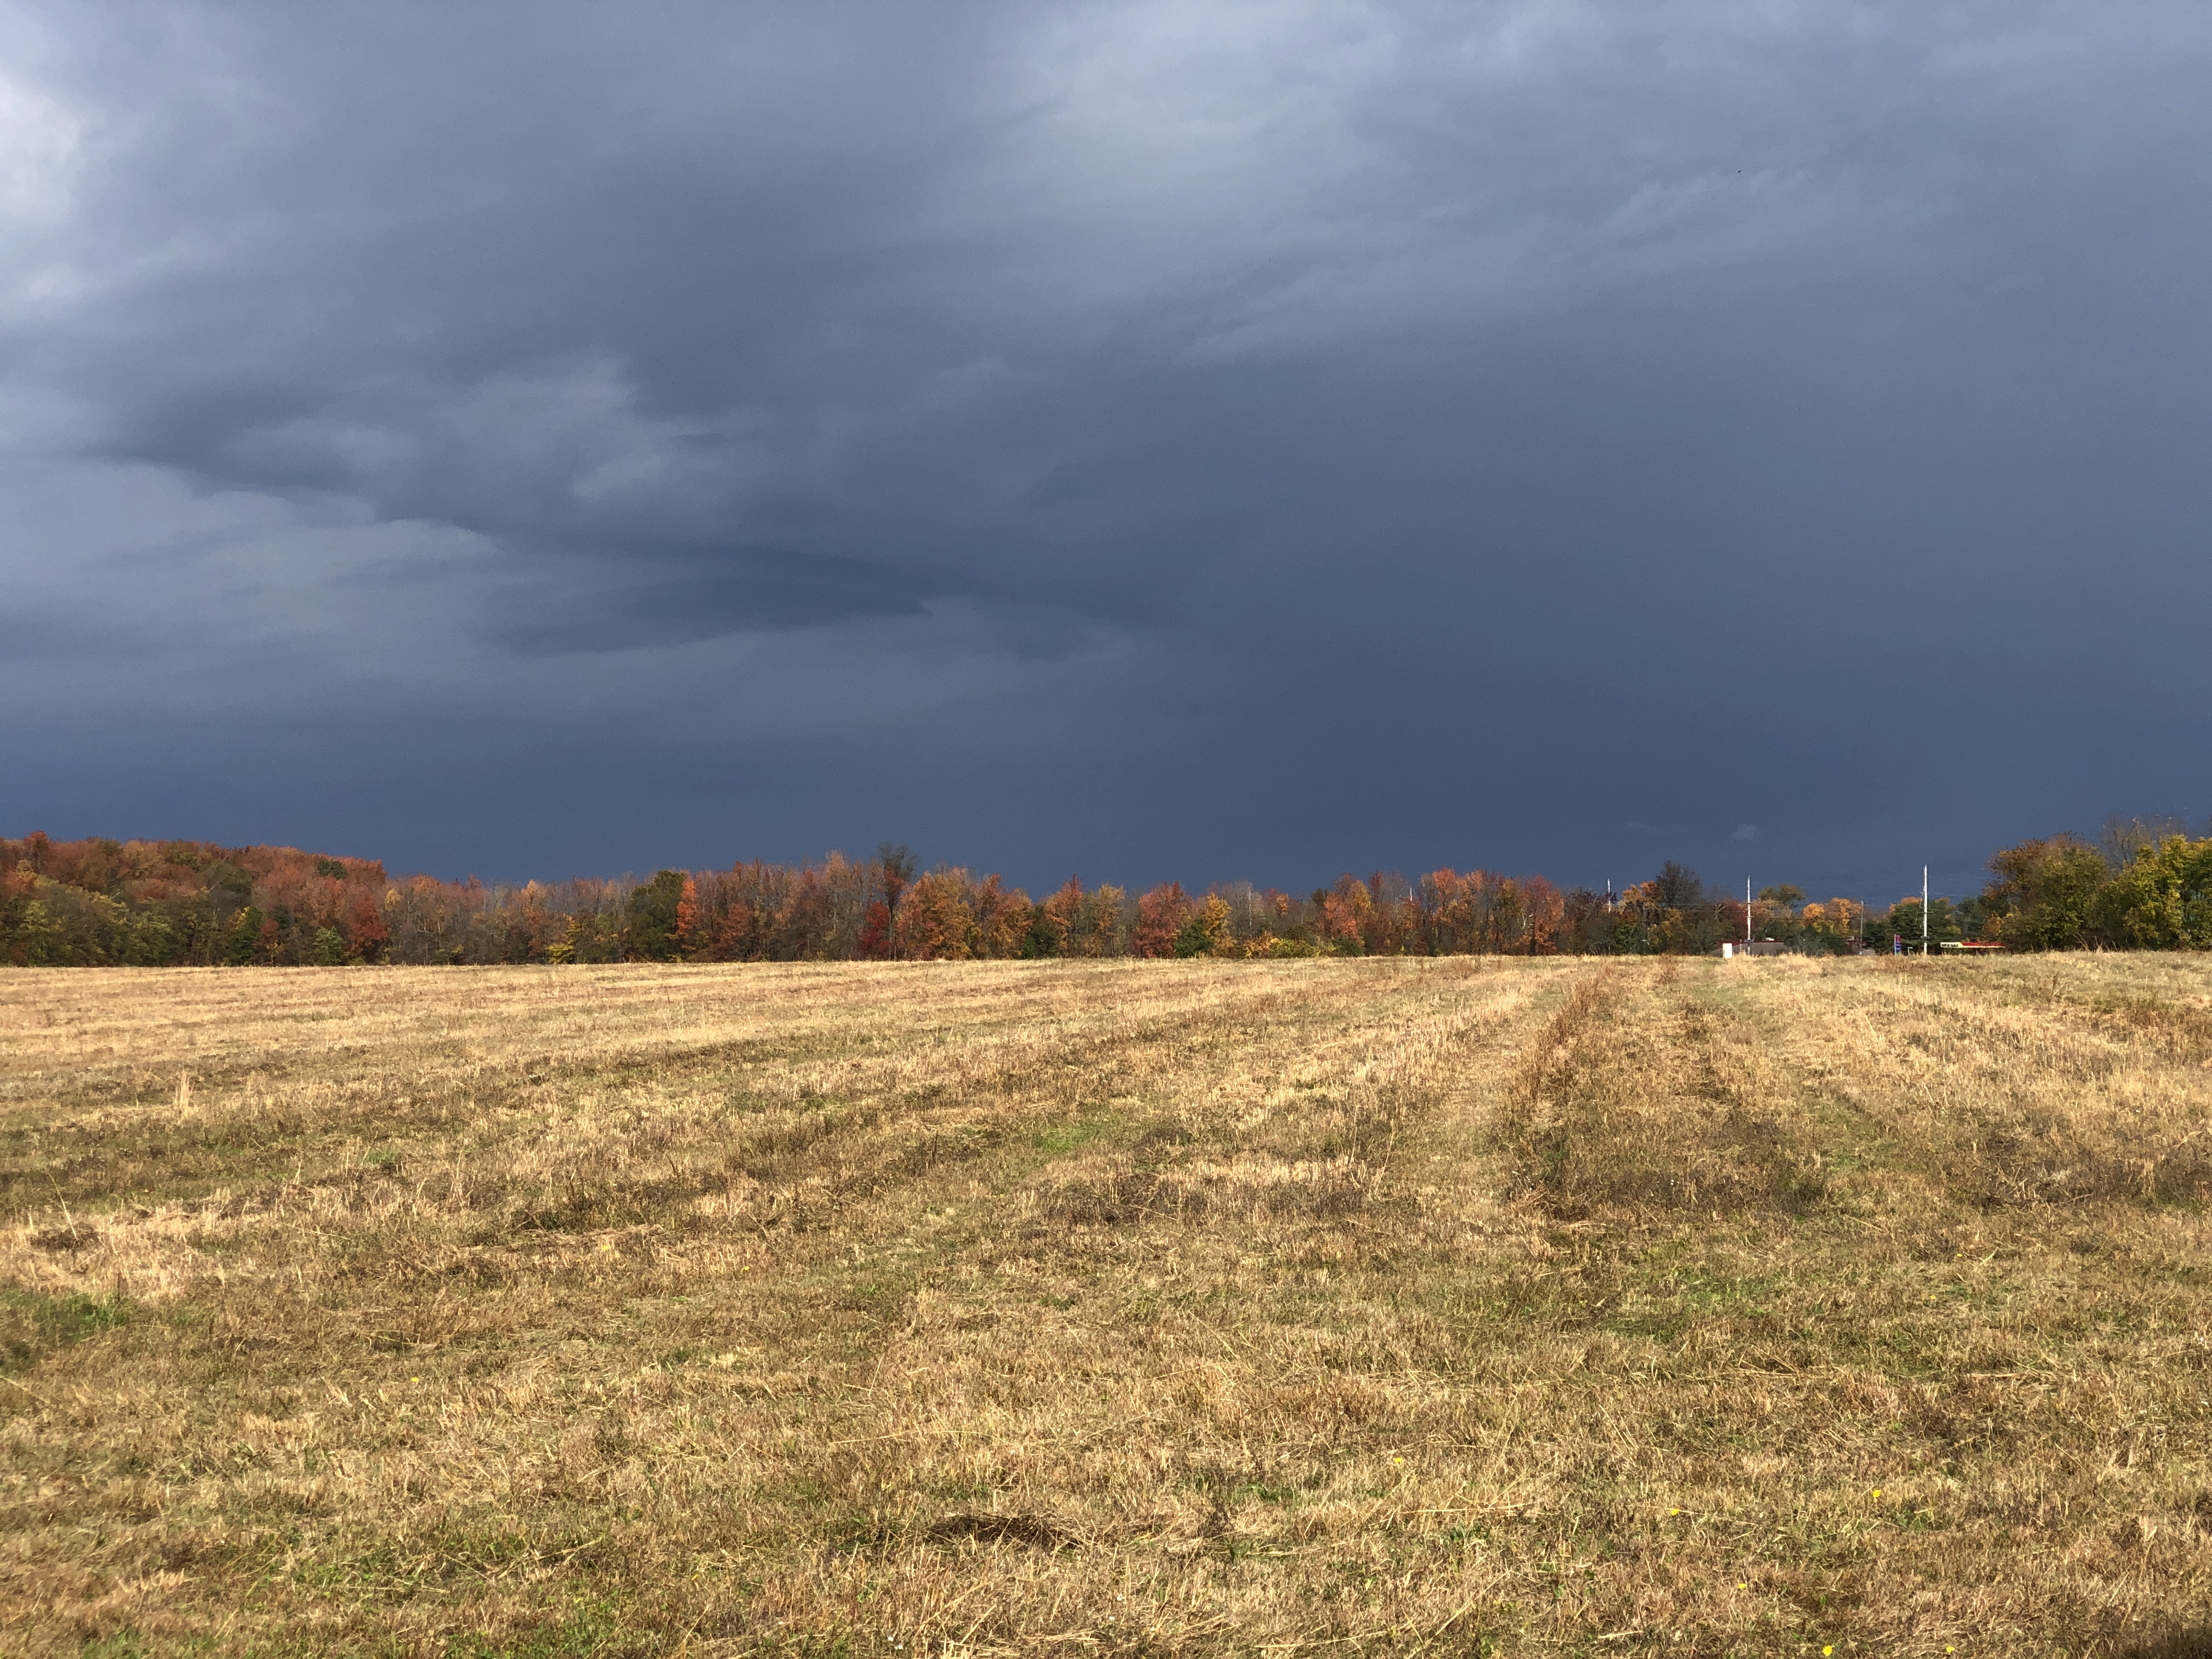
\includegraphics[height=0.9\textwidth,width=0.9\textheight,keepaspectratio=true]{clouds/nimbostratus}
    \caption{Nimbostratus}
    \label{fig:nimbostratus}
    % https://commons.wikimedia.org/wiki/File:2023-10-29_12_25_34_View_towards_dark_clouds_from_Burlington_County_Route_630_(Woodlane_Road)_in_Westampton_Township,_Burlington_County,_New_Jersey.jpg
  \end{sidewaysfigure*}
  
  \begin{sidewaysfigure*}
    \centering
    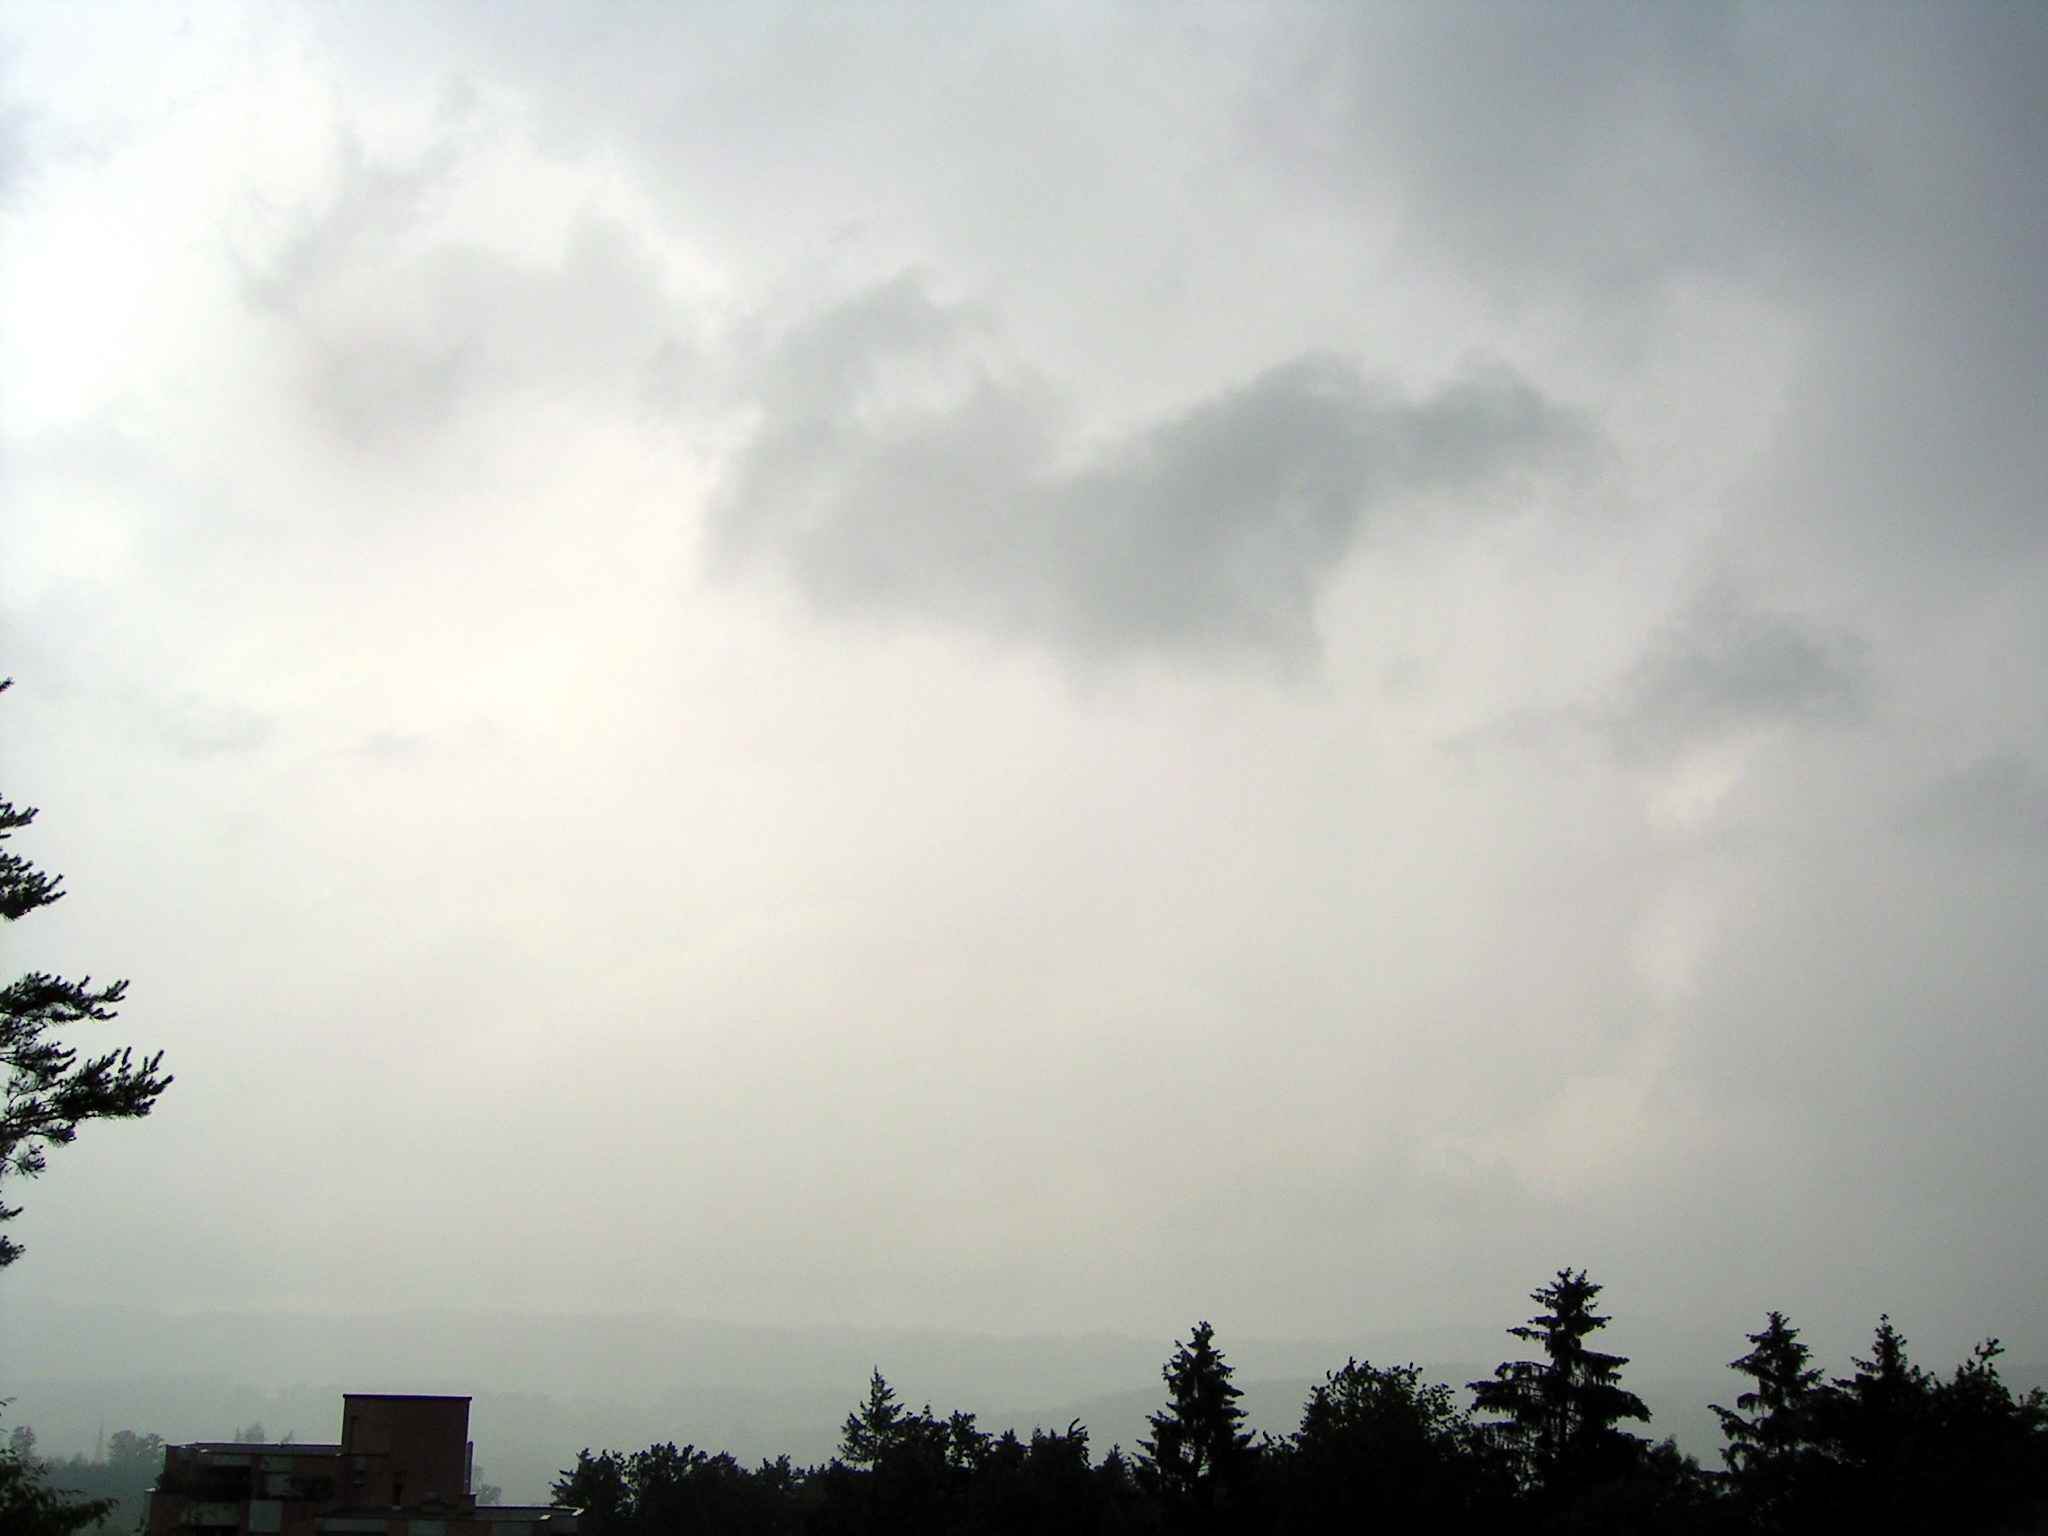
\includegraphics[width=0.9\textheight,keepaspectratio=true]{clouds/fractostratus_over_nimbostratus}
    \caption{Fractostratus на фоне Nimbostratus}
    \label{fig:fractostratus}
    % https://commons.wikimedia.org/wiki/File:Ns1.jpg
  \end{sidewaysfigure*}

  \begin{sidewaysfigure*}
    \centering
    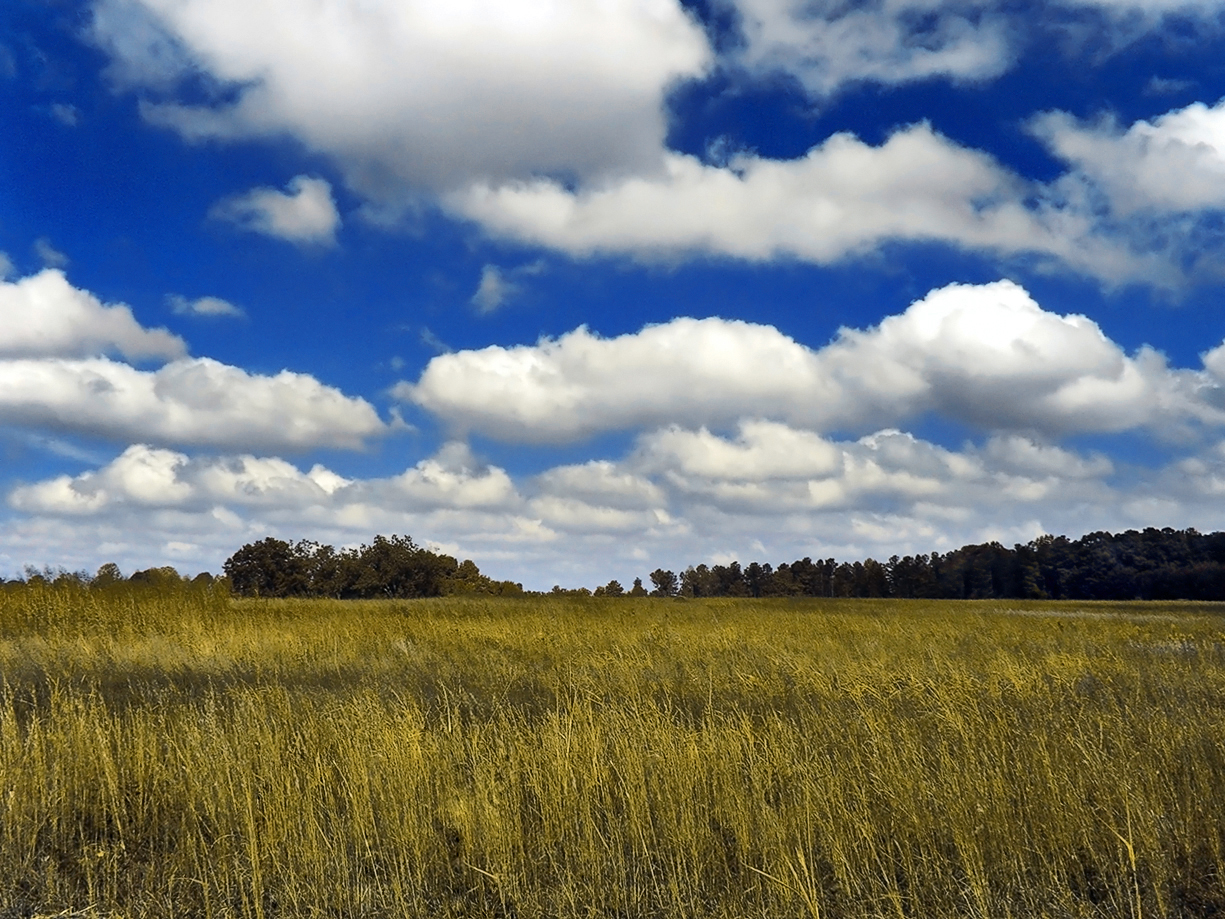
\includegraphics[width=0.9\textheight,keepaspectratio=true]{clouds/cumulus_humilis}
    \caption{Кучевые облака хорошей погоды, Cumulus humilis}
    \label{fig:112}
    % https://commons.wikimedia.org/wiki/File:GoldenMedows.jpg
  \end{sidewaysfigure*}

  \begin{figure*}
    \centering
    \includegraphics[width=0.9\textwidth,keepaspectratio=true]{clouds/cumulonimbus}
    \caption{Кучево-дождевое облако (<<наковальня>>), Cumulonimbus calvus}
    \label{fig:113}
    % https://commons.wikimedia.org/wiki/File:Sunnystormcloud.jpg
  \end{figure*}

  \begin{sidewaysfigure*}
    \centering
    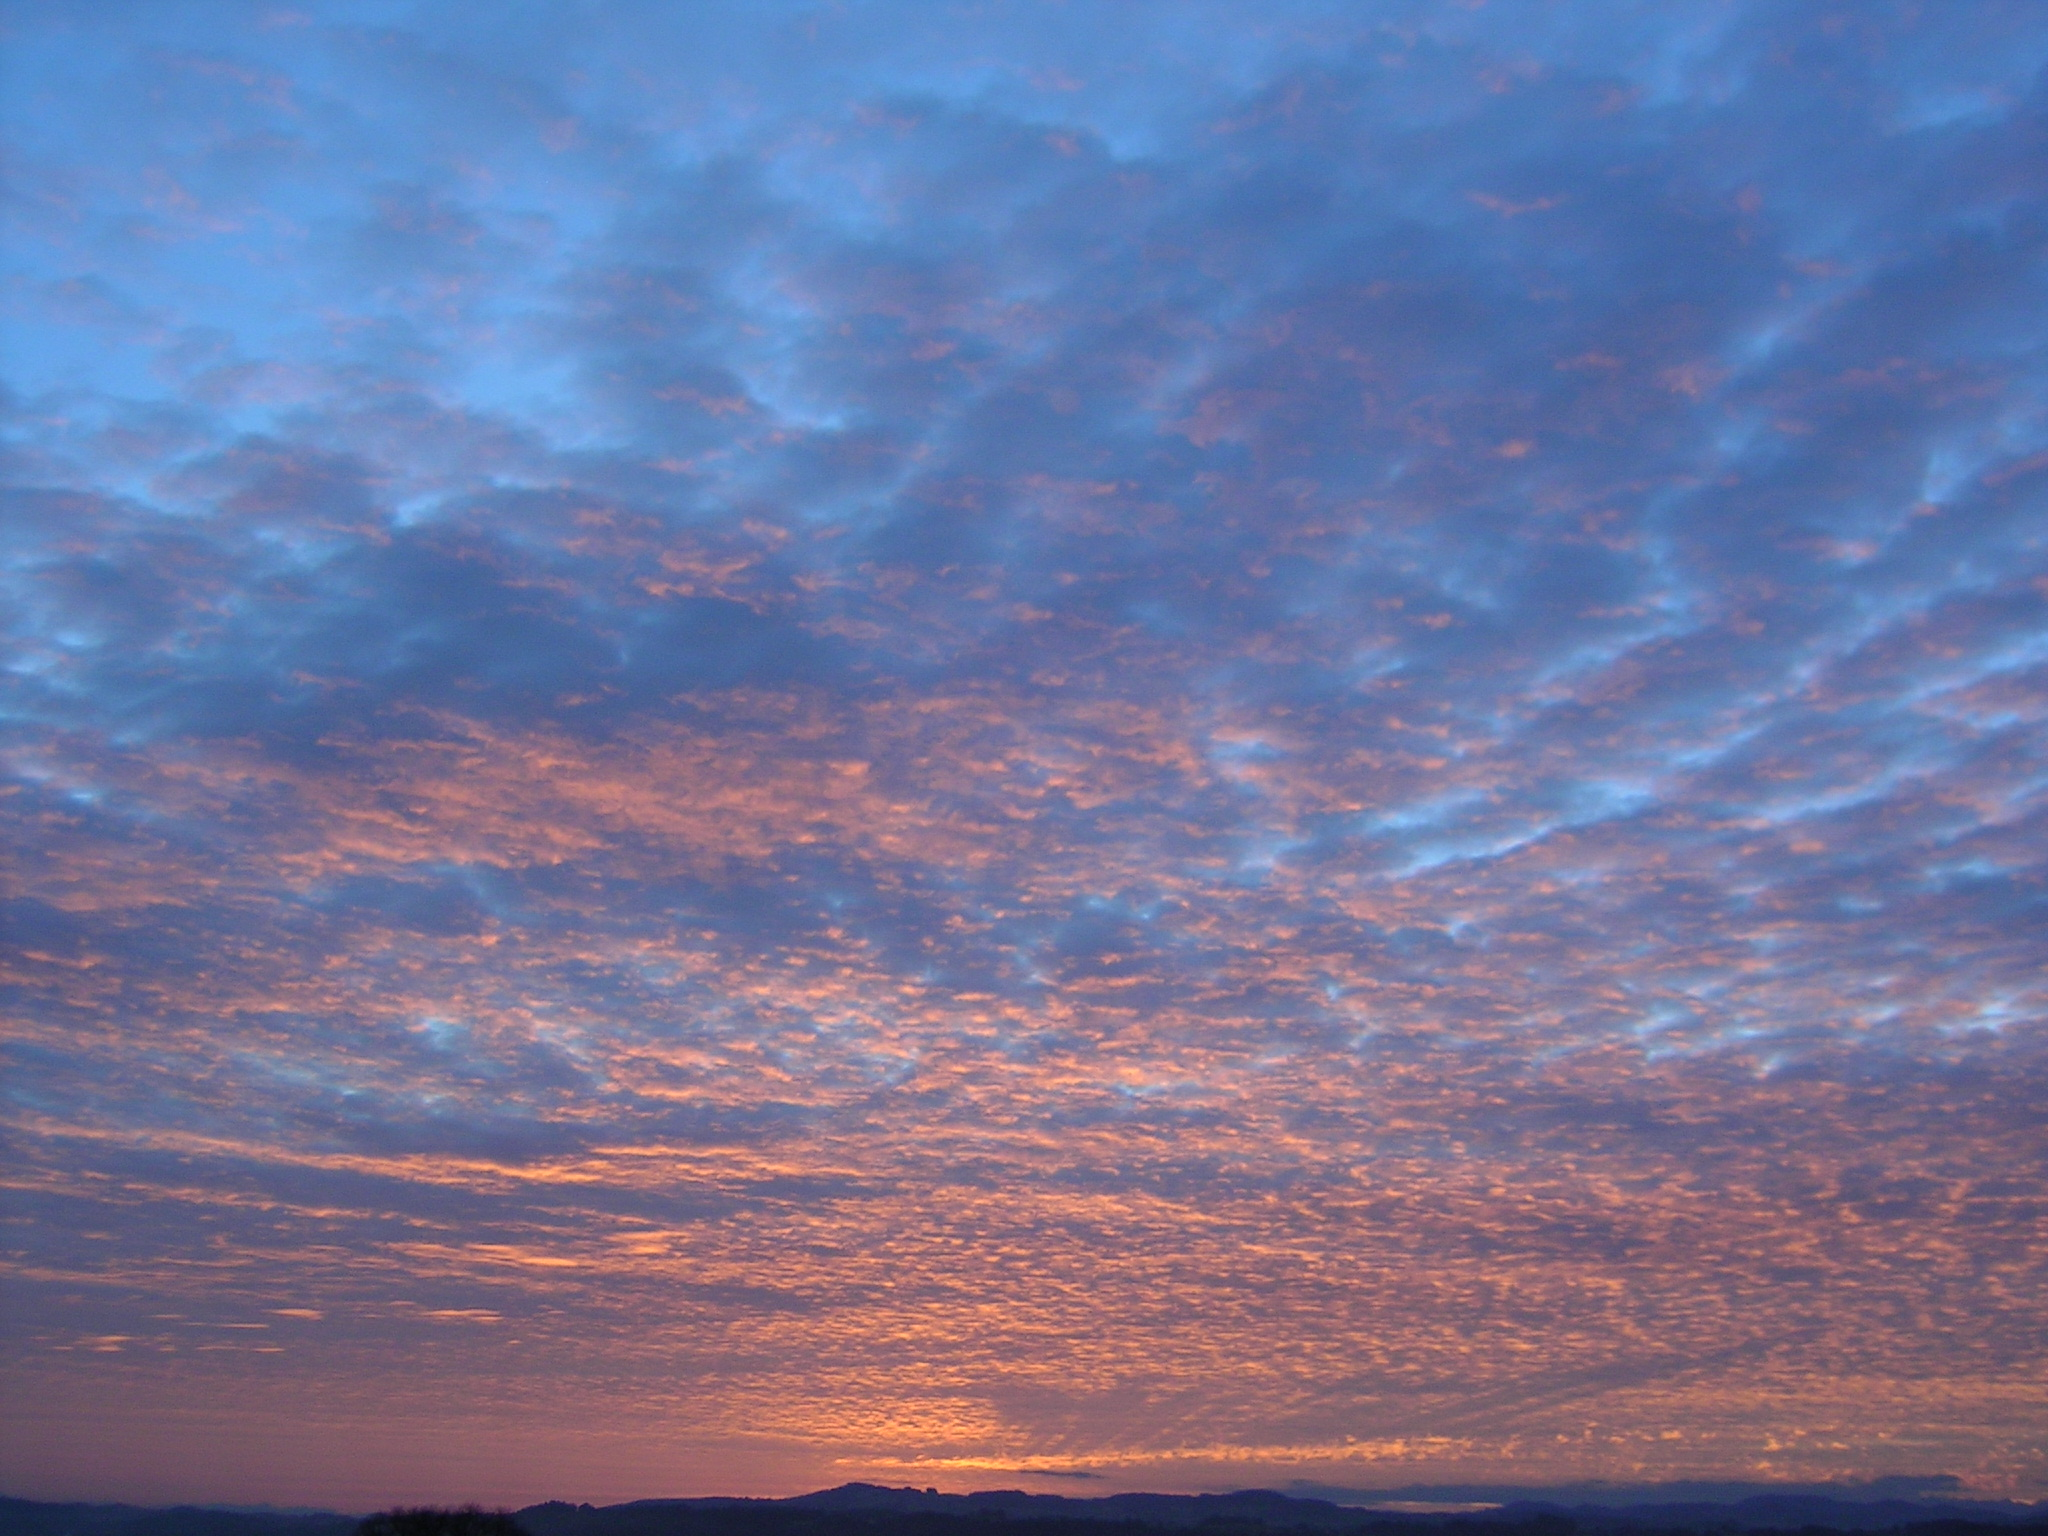
\includegraphics[width=0.9\textheight,keepaspectratio=true]{clouds/altocumulus}
    \caption{Высококучевые облака (<<барашки>>), Altocumulus}
    \label{fig:114}
    % https://commons.wikimedia.org/wiki/File:Partially_illuminated_Ac_with_shadows.JPG
  \end{sidewaysfigure*}

  \begin{sidewaysfigure*}
    \centering
    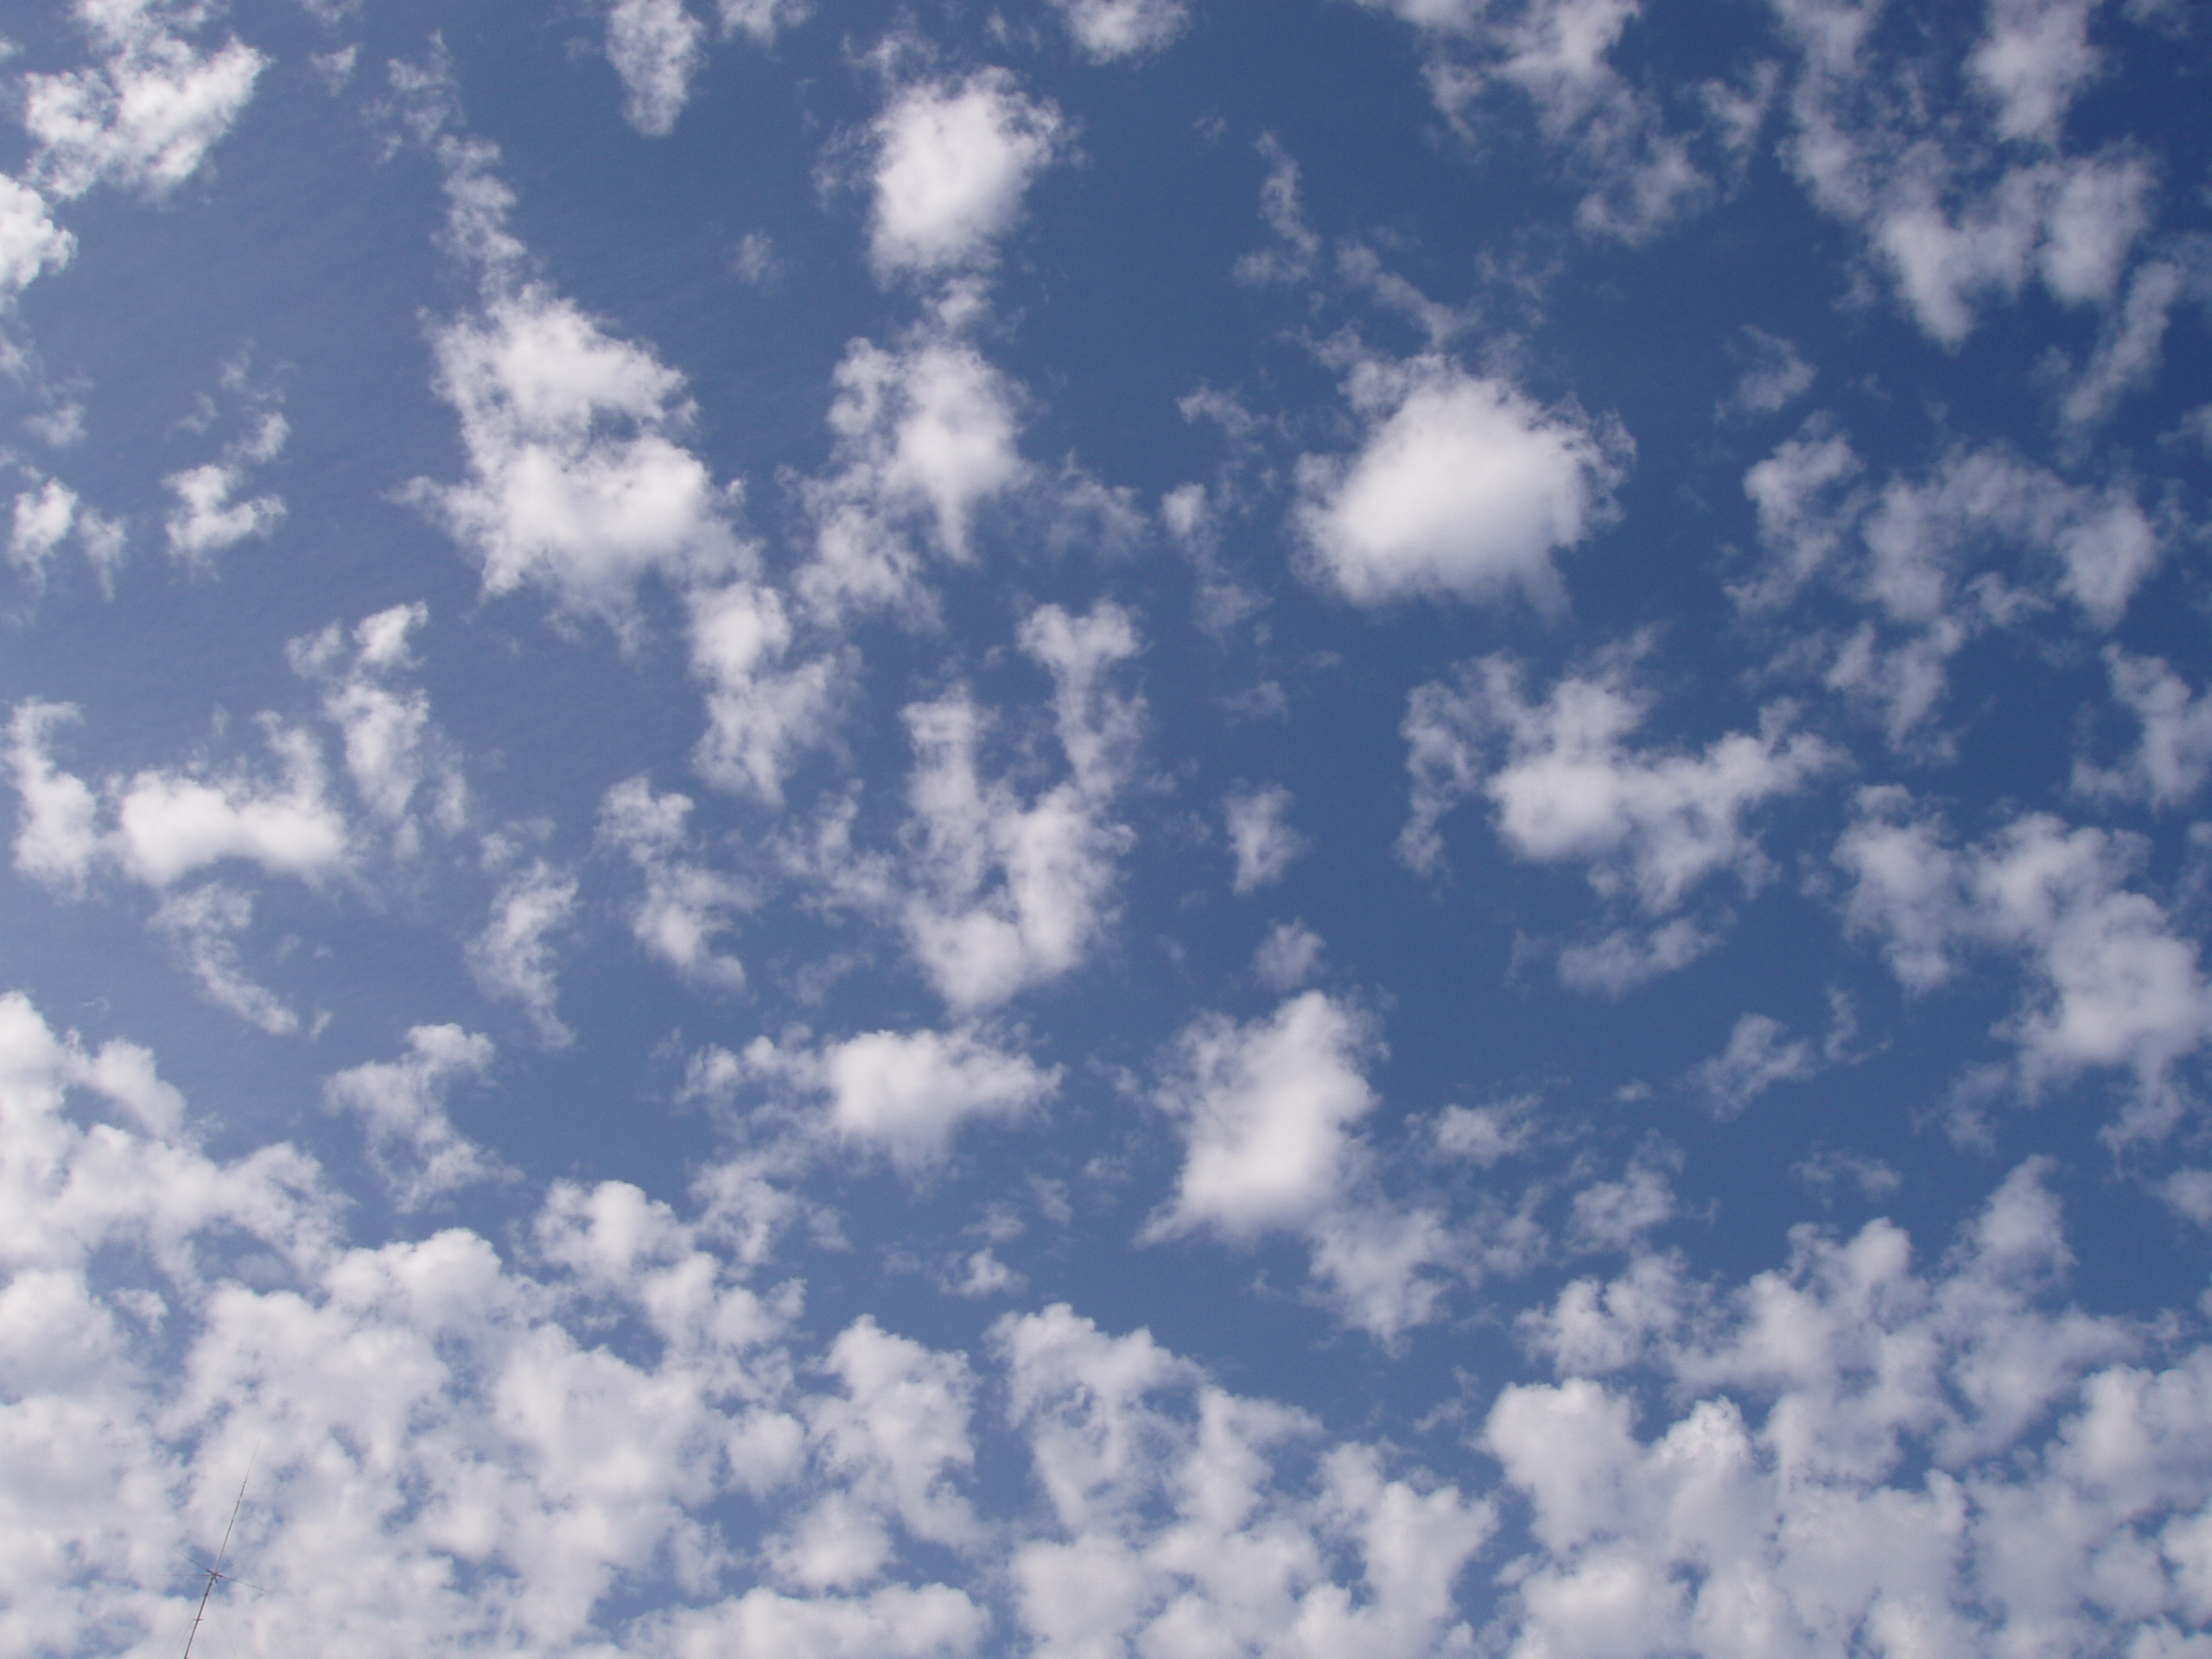
\includegraphics[width=0.9\textheight,keepaspectratio=true]{clouds/altocumulus1}
    \caption{Altocumulus}
    \label{fig:altocumulus-1}
    % https://commons.wikimedia.org/wiki/File:Altocumulus_cloud.jpg
  \end{sidewaysfigure*}

  \begin{sidewaysfigure*}
    \centering
    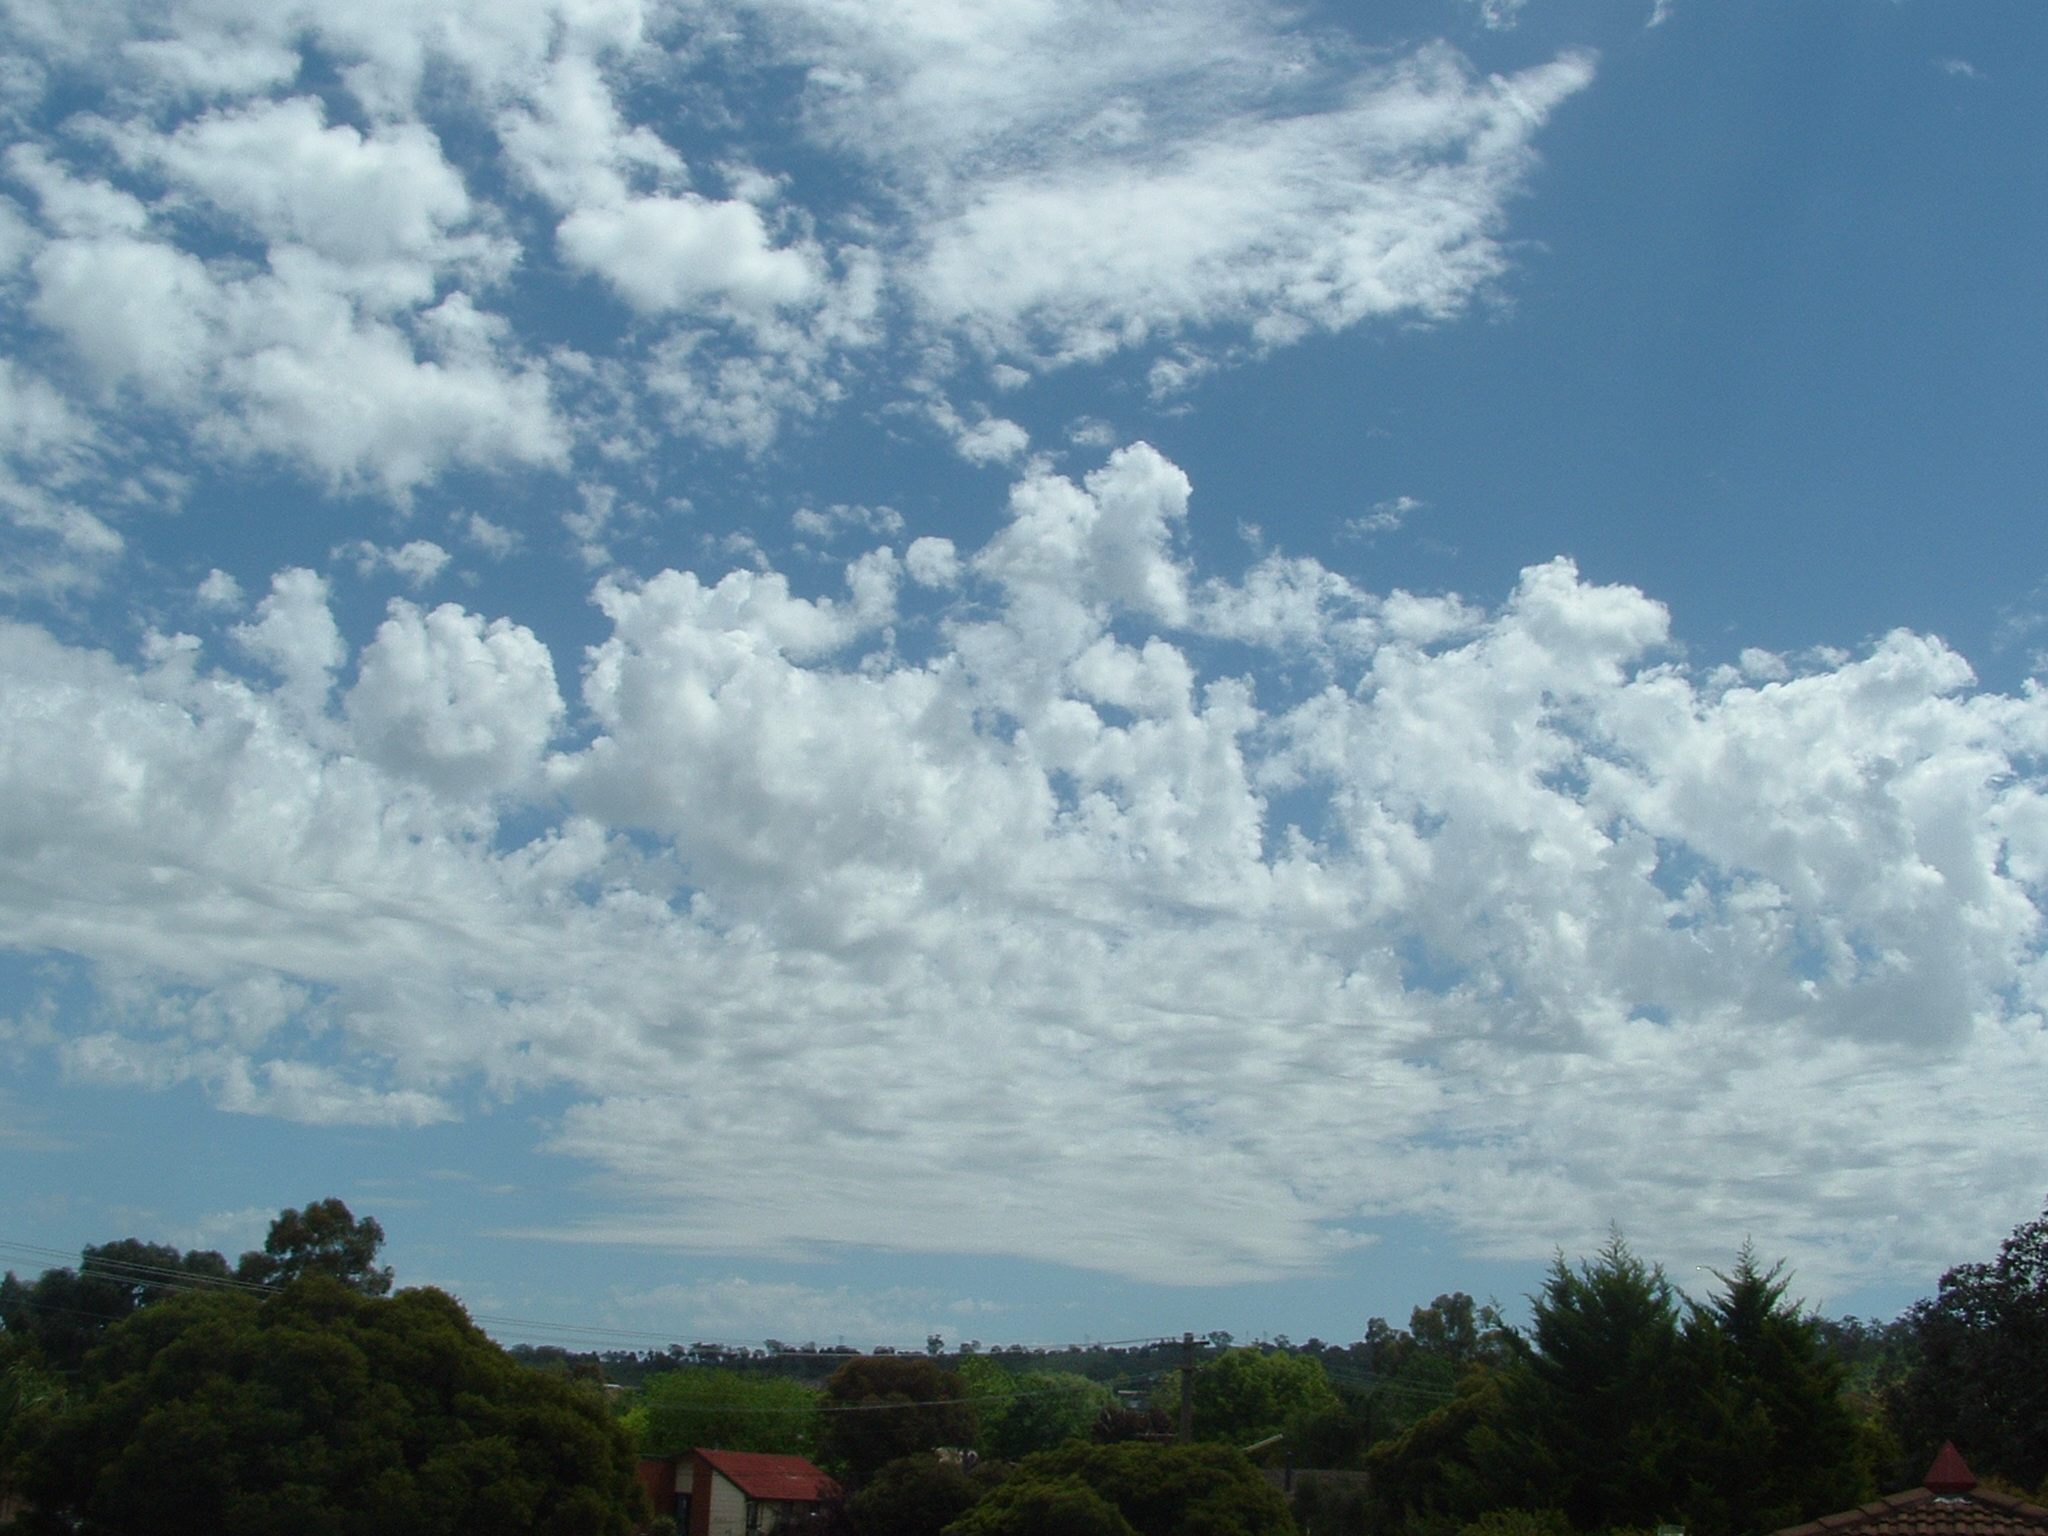
\includegraphics[width=0.9\textheight,keepaspectratio=true]{clouds/altocumulus_castellanus}
    \caption{Altocumulus}
    \label{fig:altocumulus-castellanus}
    % https://it.m.wikipedia.org/wiki/File:Altocumulus-Castellanus.jpg
  \end{sidewaysfigure*}

  \begin{sidewaysfigure*}
    \centering
    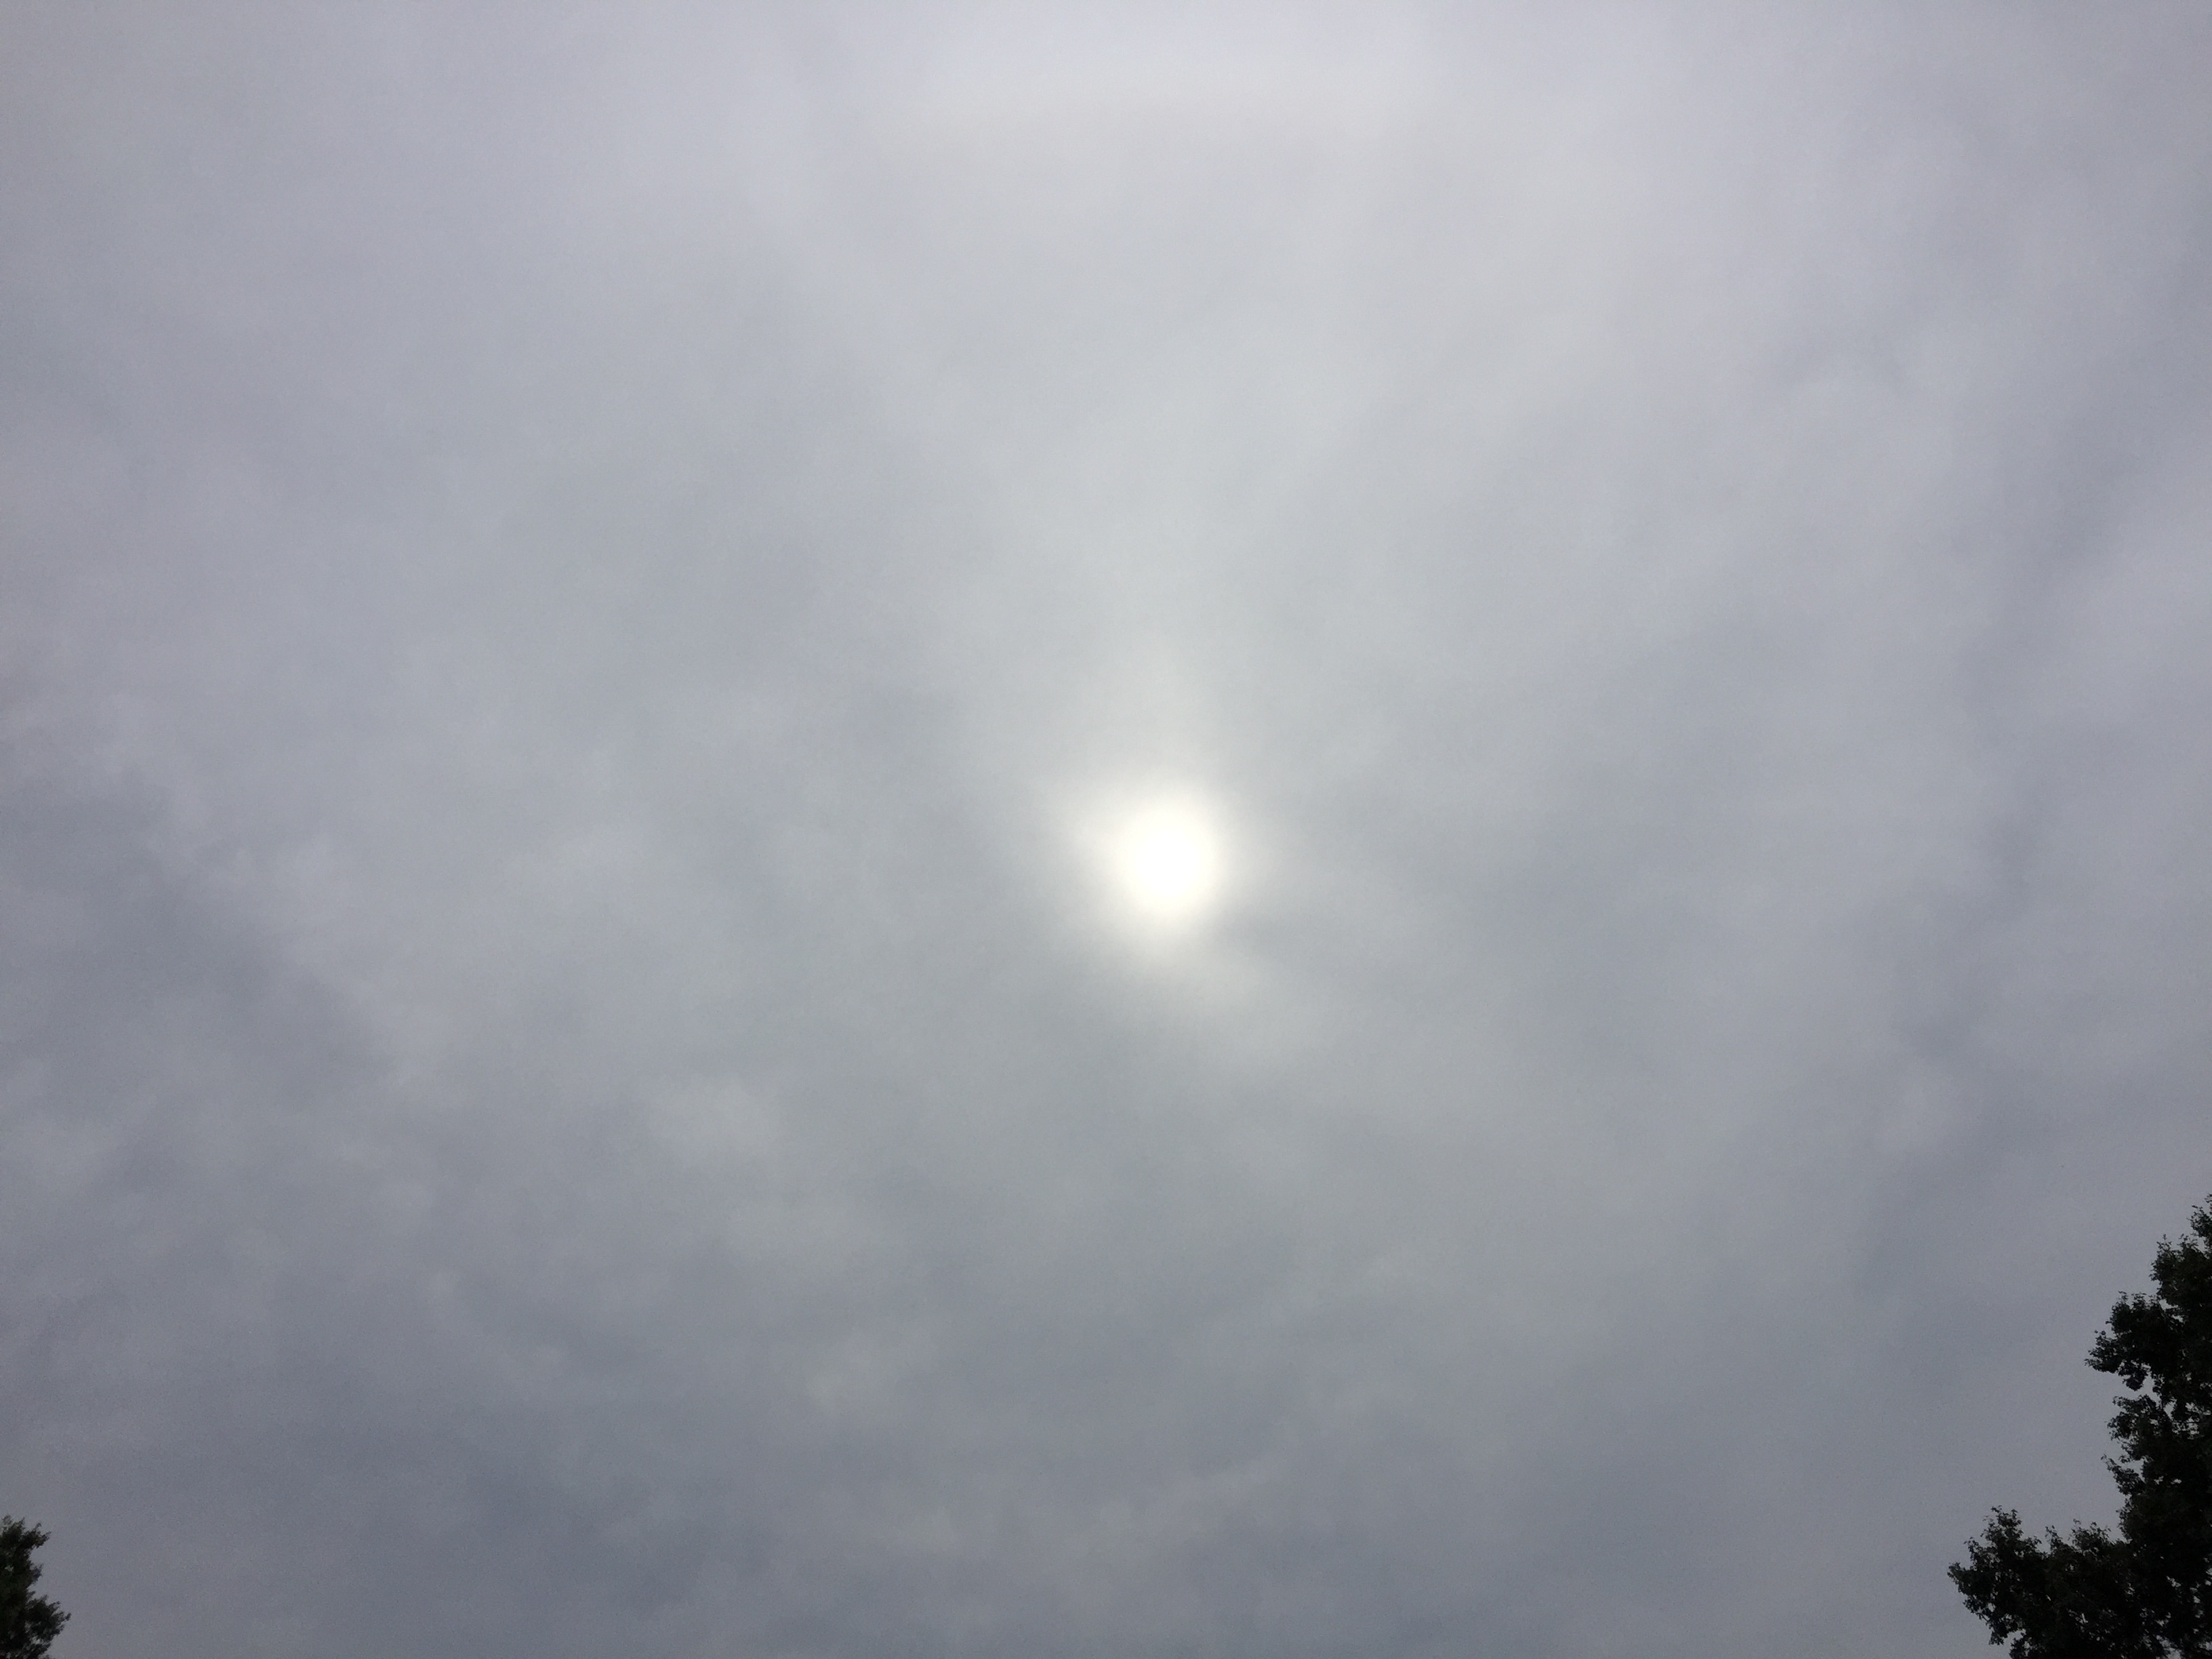
\includegraphics[width=0.9\textheight,keepaspectratio=true]{clouds/altostratus_translucidus}
    \caption{Солнце просвечивает через Altostratus translucidus}
    \label{fig:altostratus-translucidus}
    % https://commons.wikimedia.org/wiki/File:2017-06-22_16_57_51_Sun_shining_dimly_through_an_altostratus_cloud_layer_over_Ladybank_Lane_in_the_Chantilly_Highlands_section_of_Oak_Hill,_Fairfax_County,_Virginia.jpg
  \end{sidewaysfigure*}

  \begin{sidewaysfigure*}
    \centering
    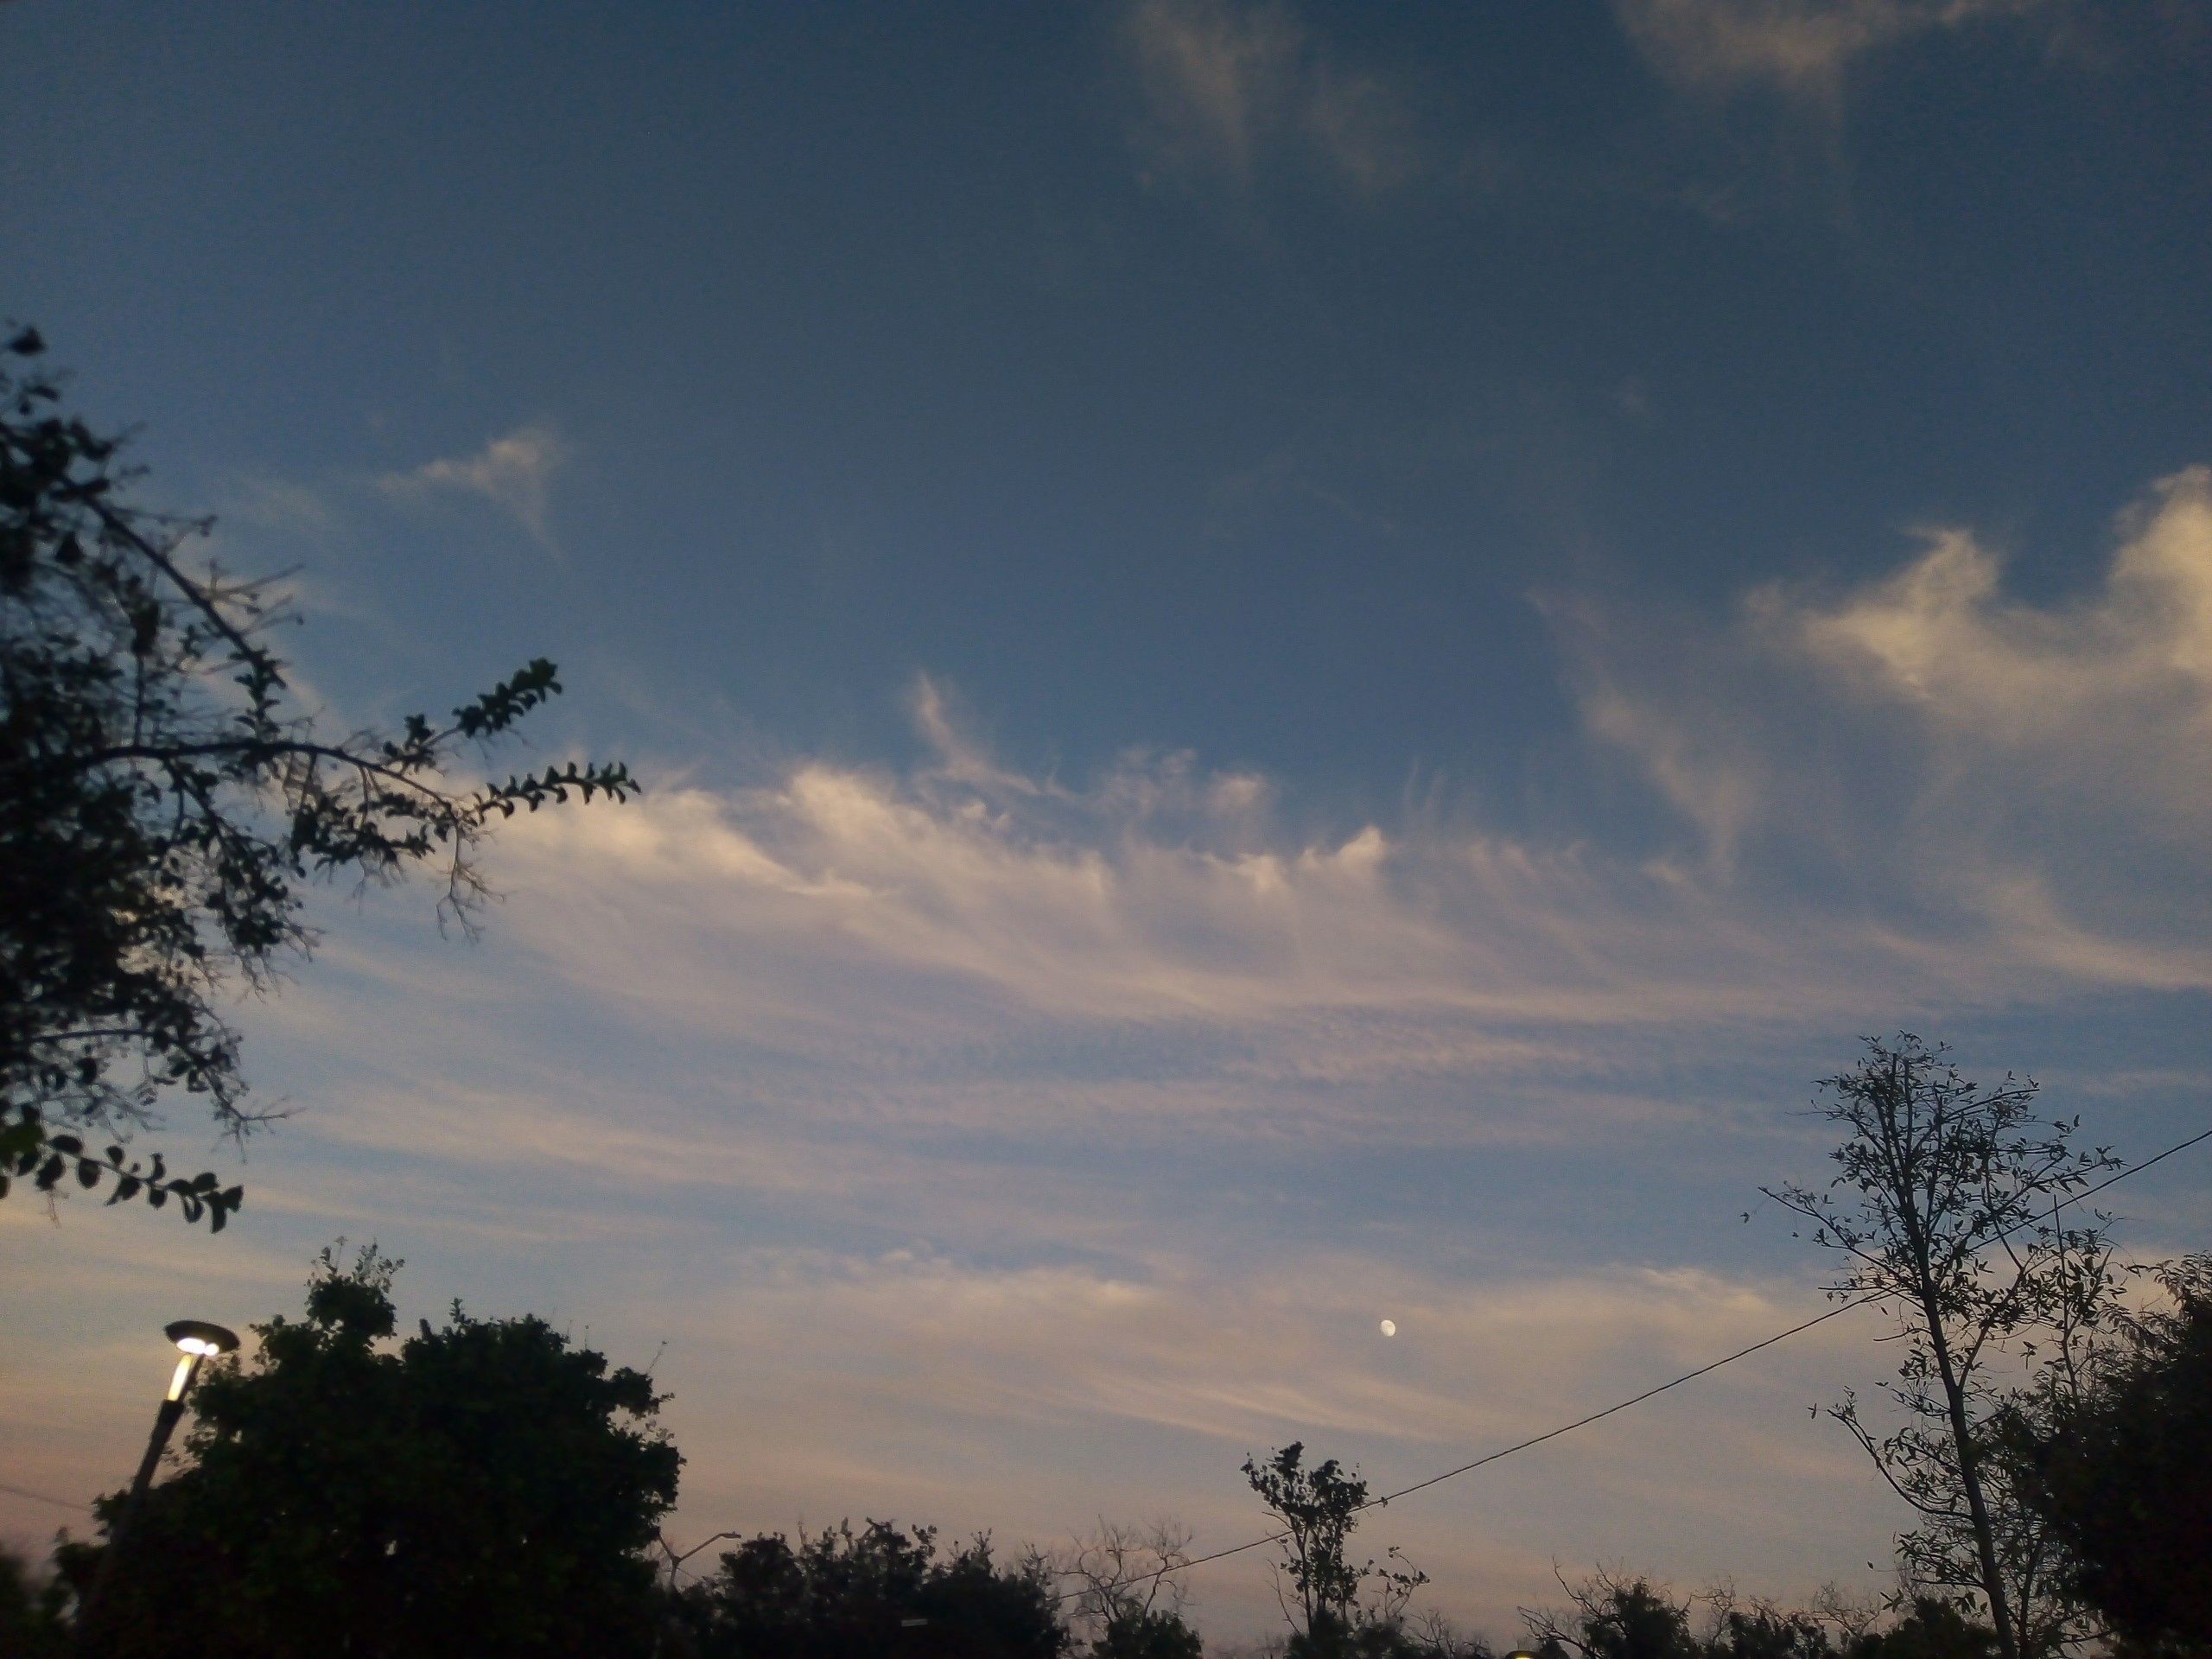
\includegraphics[width=0.9\textheight,keepaspectratio=true]{clouds/cirrus_floccus}
    \caption{Перистые облака, Cirrus flocus}
    \label{fig:115}
    % https://commons.wikimedia.org/wiki/File:Cirrus_floccus_with_virga_001.jpg
  \end{sidewaysfigure*}

  \begin{sidewaysfigure*}
    \centering{}
    % https://upload.wikimedia.org/wikipedia/commons/f/f0/Cirrus_front_over_Austnesfjorden%2C_Austv%C3%A5g%C3%B8ya%2C_Lofoten%2C_Norway%2C_2015_April.jpg
    \includegraphics[width=0.9\textheight,keepaspectratio=true]{clouds/cirrus_fibratus.jpeg}
    \caption{Перистые нитевидные, Cirrus fibratus}
    \label{fig:pp01-1}
  \end{sidewaysfigure*}

  \begin{sidewaysfigure*}
    \centering{}
    % https://commons.wikimedia.org/wiki/File:Cirrus_clouds_011.jpg
    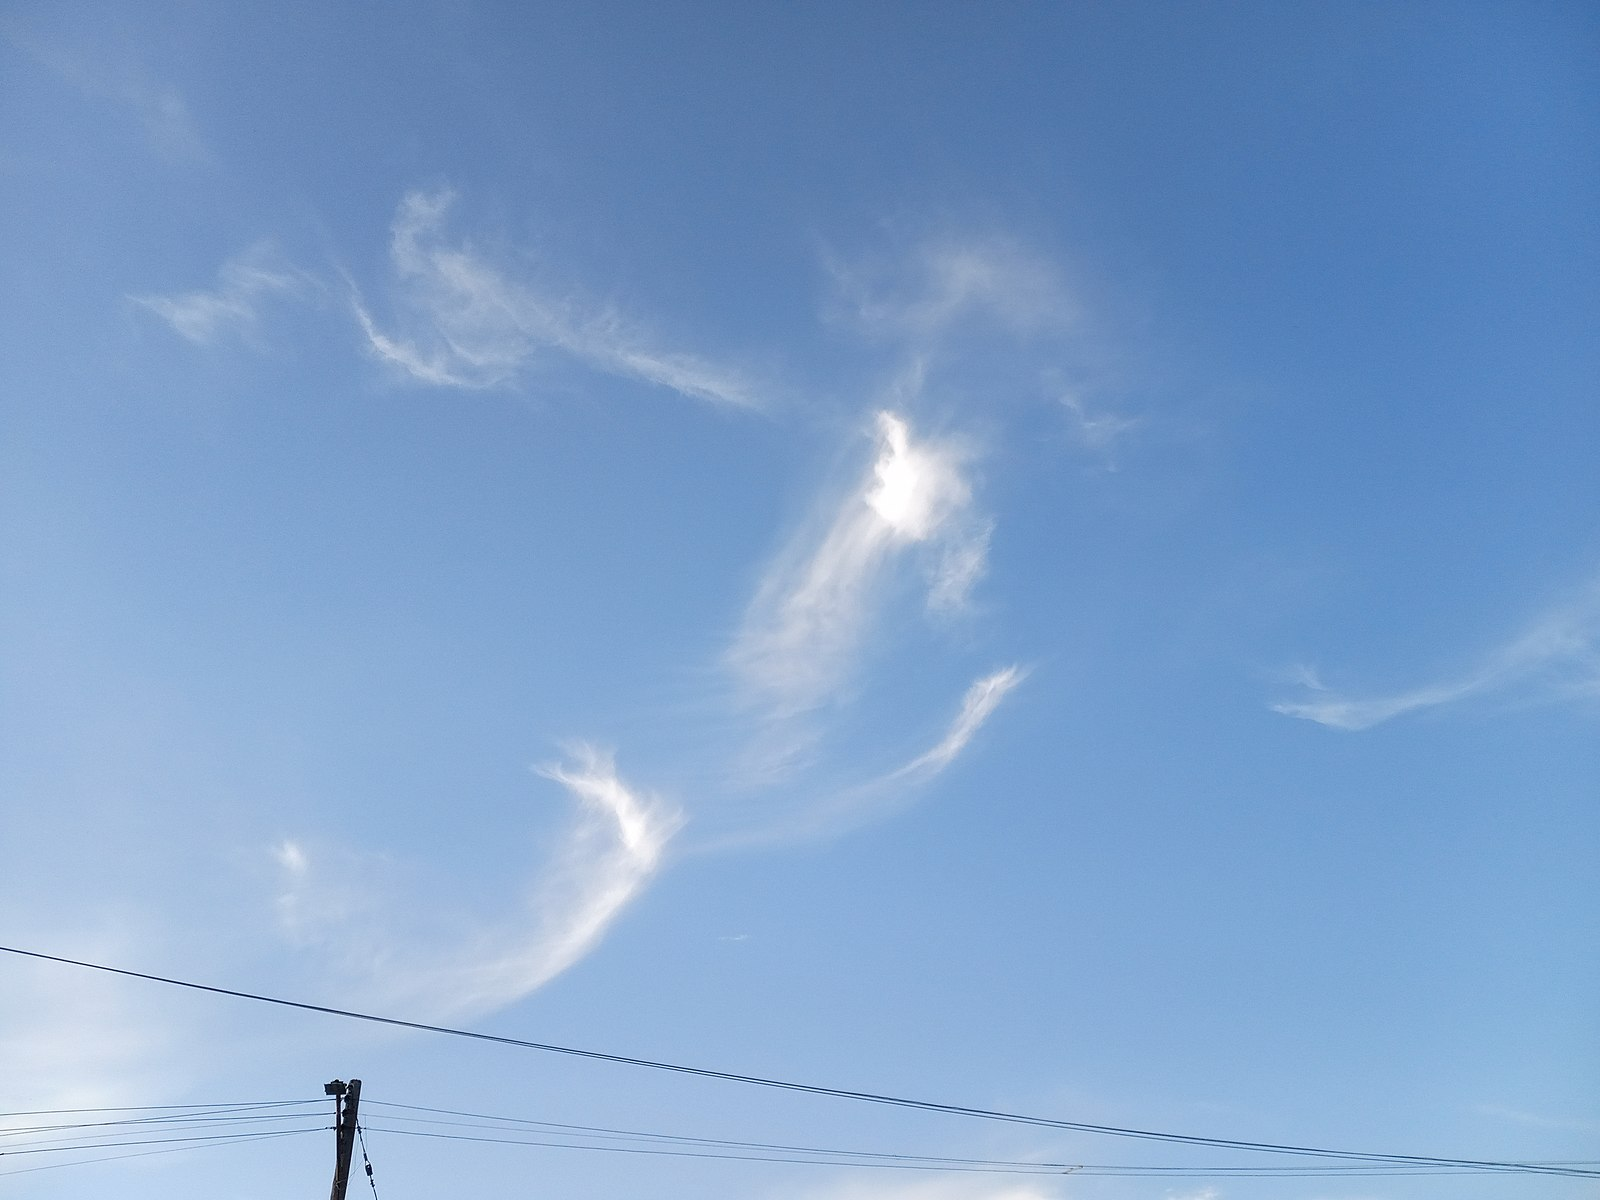
\includegraphics[width=0.9\textheight,keepaspectratio=true]{clouds/cirrus_uncinus.jpeg}
    \caption{Перистые когтевидные, Cirrus uncinus}
    \label{fig:pp01-2}
  \end{sidewaysfigure*}

  \begin{sidewaysfigure*}
    \centering
    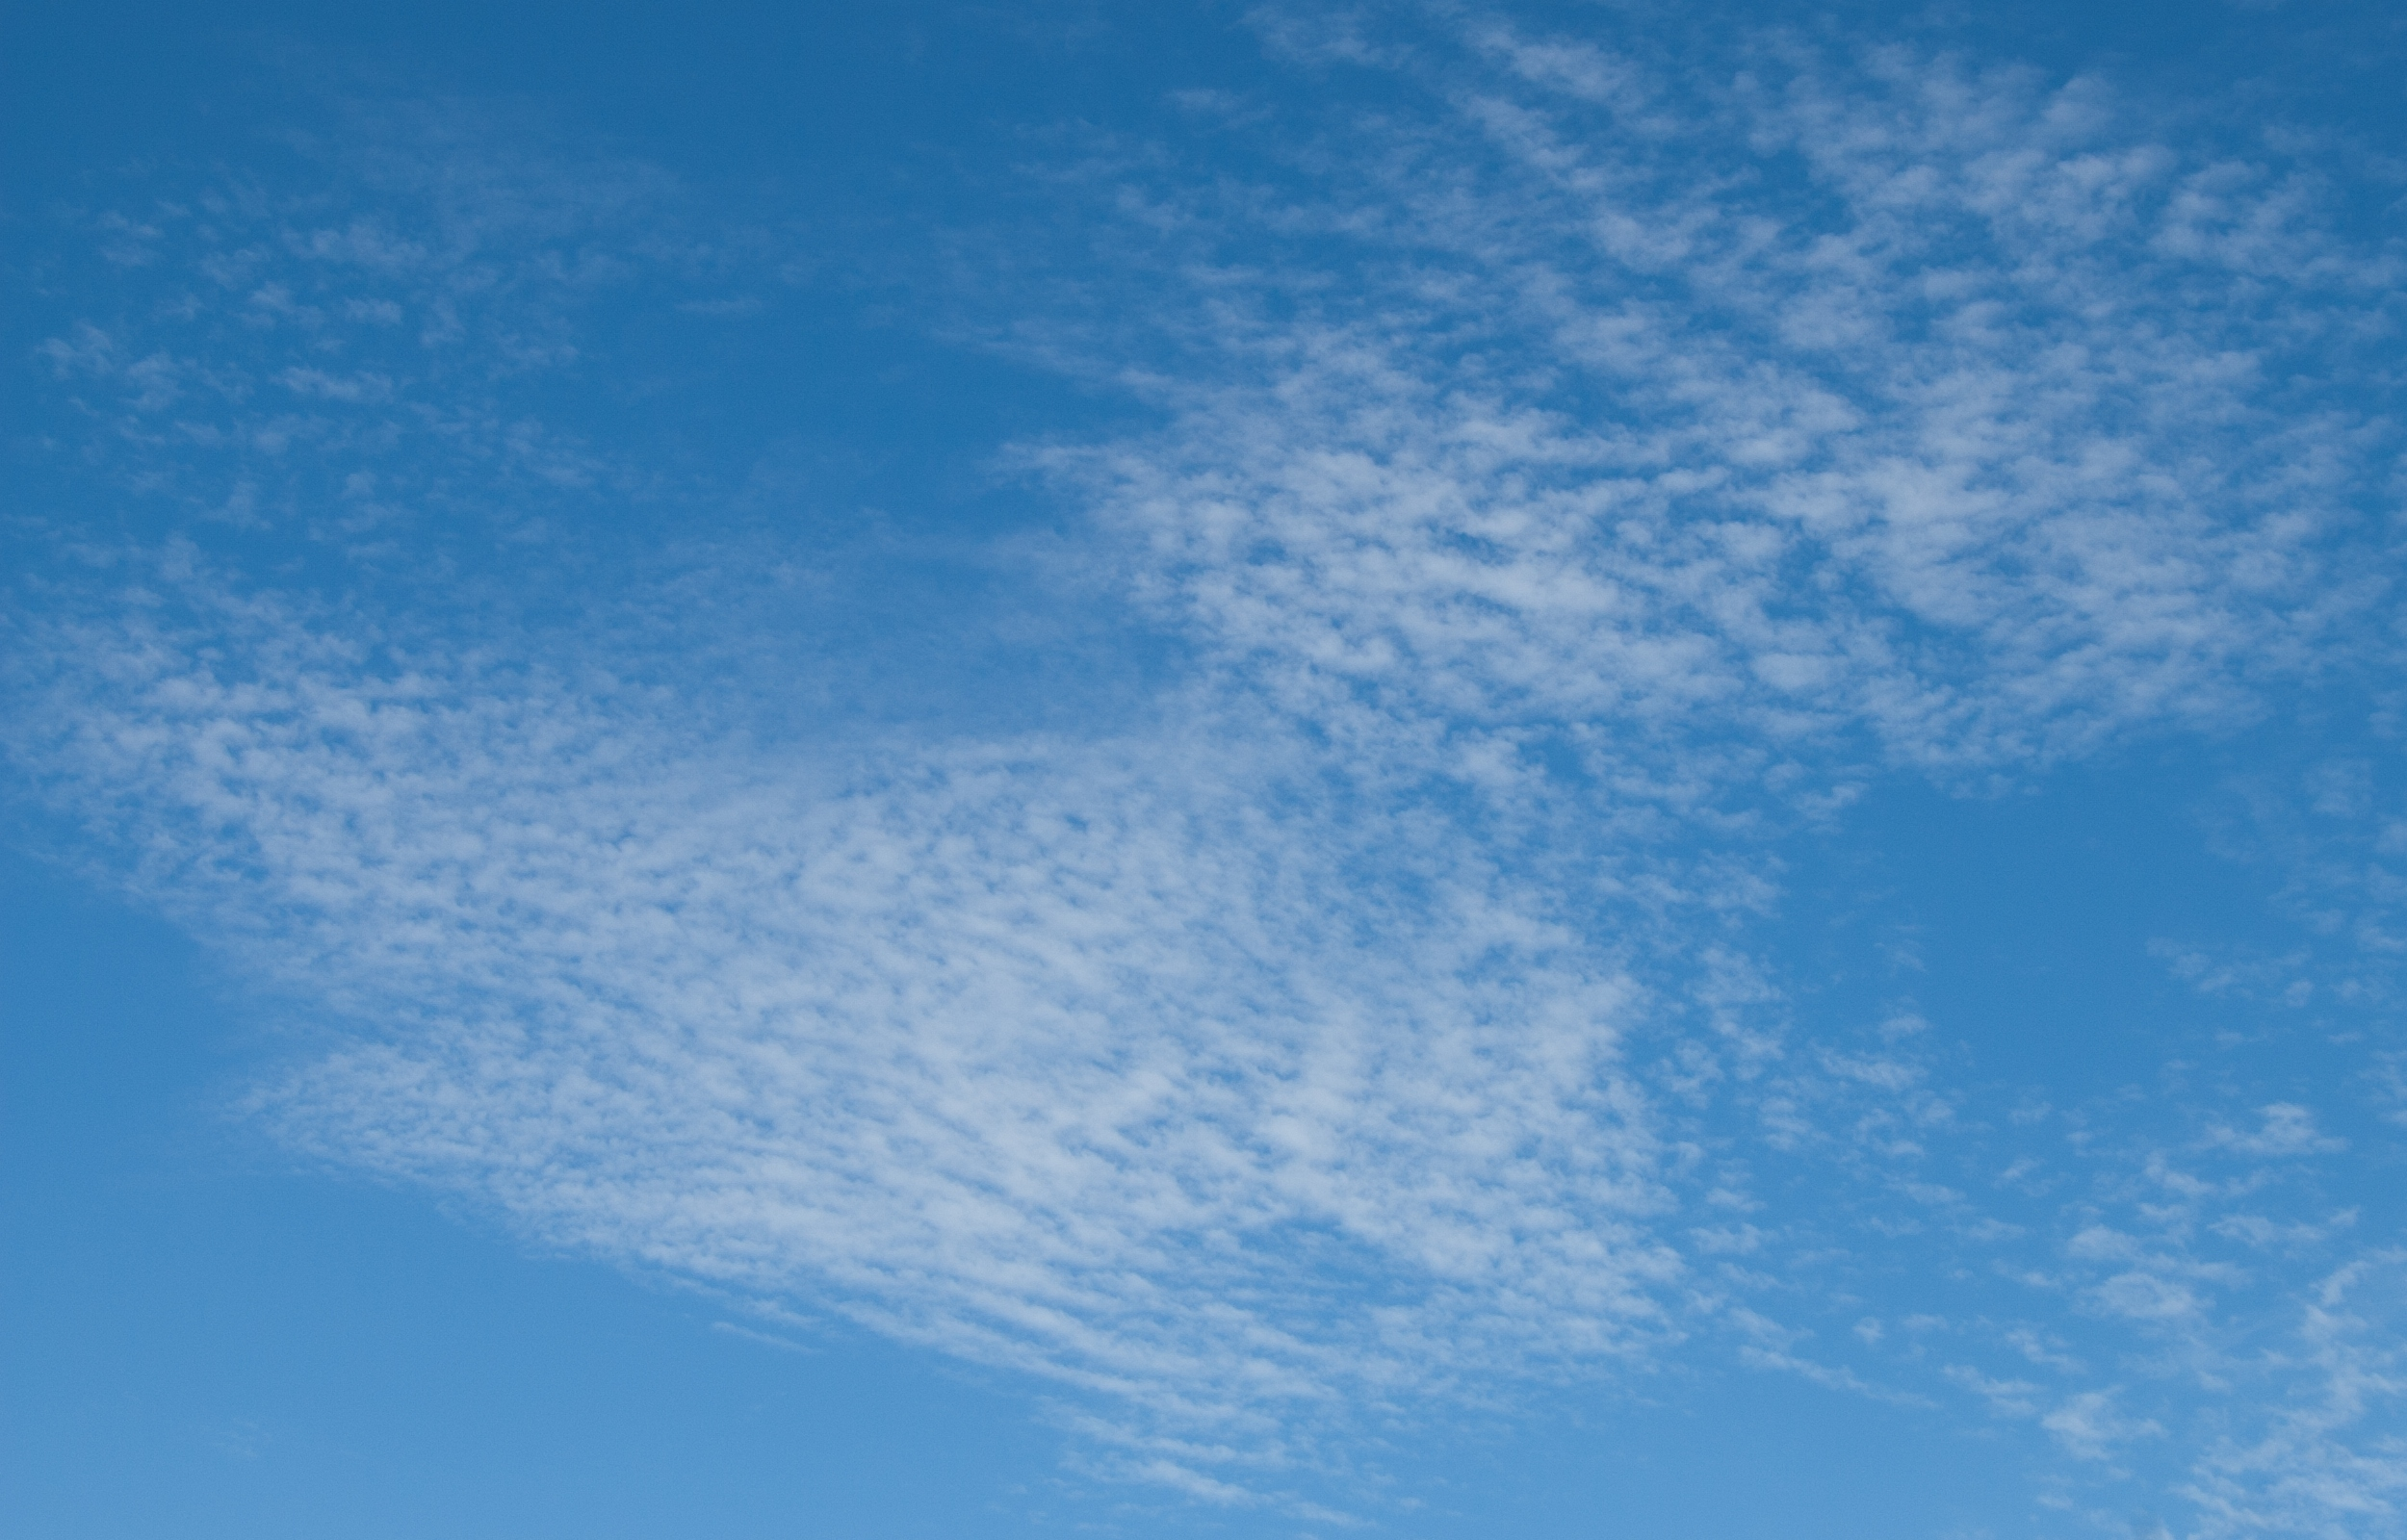
\includegraphics[width=0.9\textheight,keepaspectratio=true]{clouds/cirrocumulus}
    \caption{Перисто-кучевые, Cirrocumulus}
    \label{fig:cirrocumulus}
    % https://commons.wikimedia.org/wiki/File:Cirrocumulus_clouds_Thousand_Oaks_July_2010.jpg
  \end{sidewaysfigure*}

  \begin{sidewaysfigure*}
    \centering
    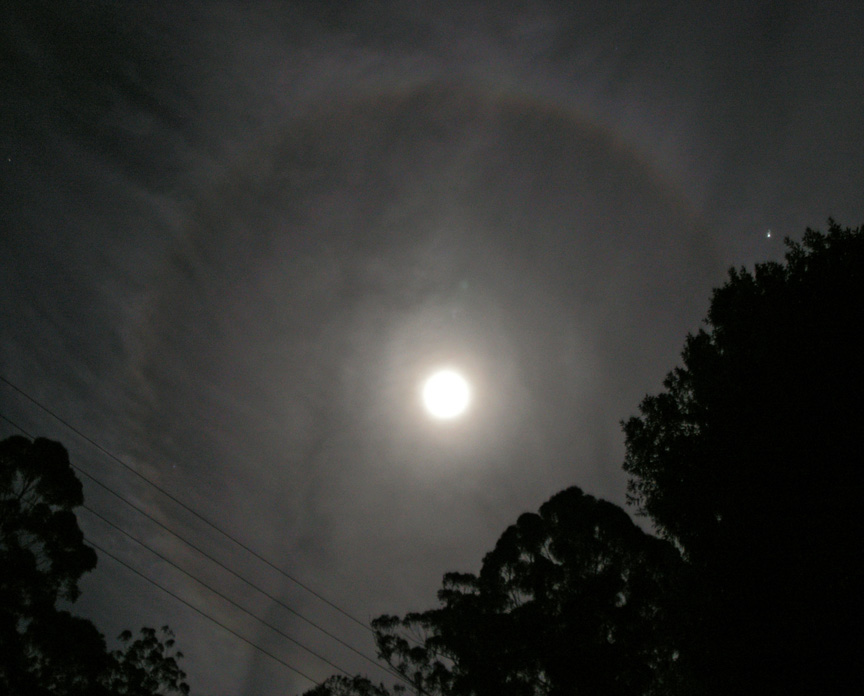
\includegraphics[width=0.9\textheight,keepaspectratio=true]{clouds/cirrostratus}
    \caption{Перисто-слоистые, Cirrostratus}
    \label{fig:cirrostratus}
    % https://commons.wikimedia.org/wiki/File:MoonHaloDonnellyMillsWA_2005_SeanMcClean.jpg
  \end{sidewaysfigure*}

  \begin{sidewaysfigure*}
    \centering
    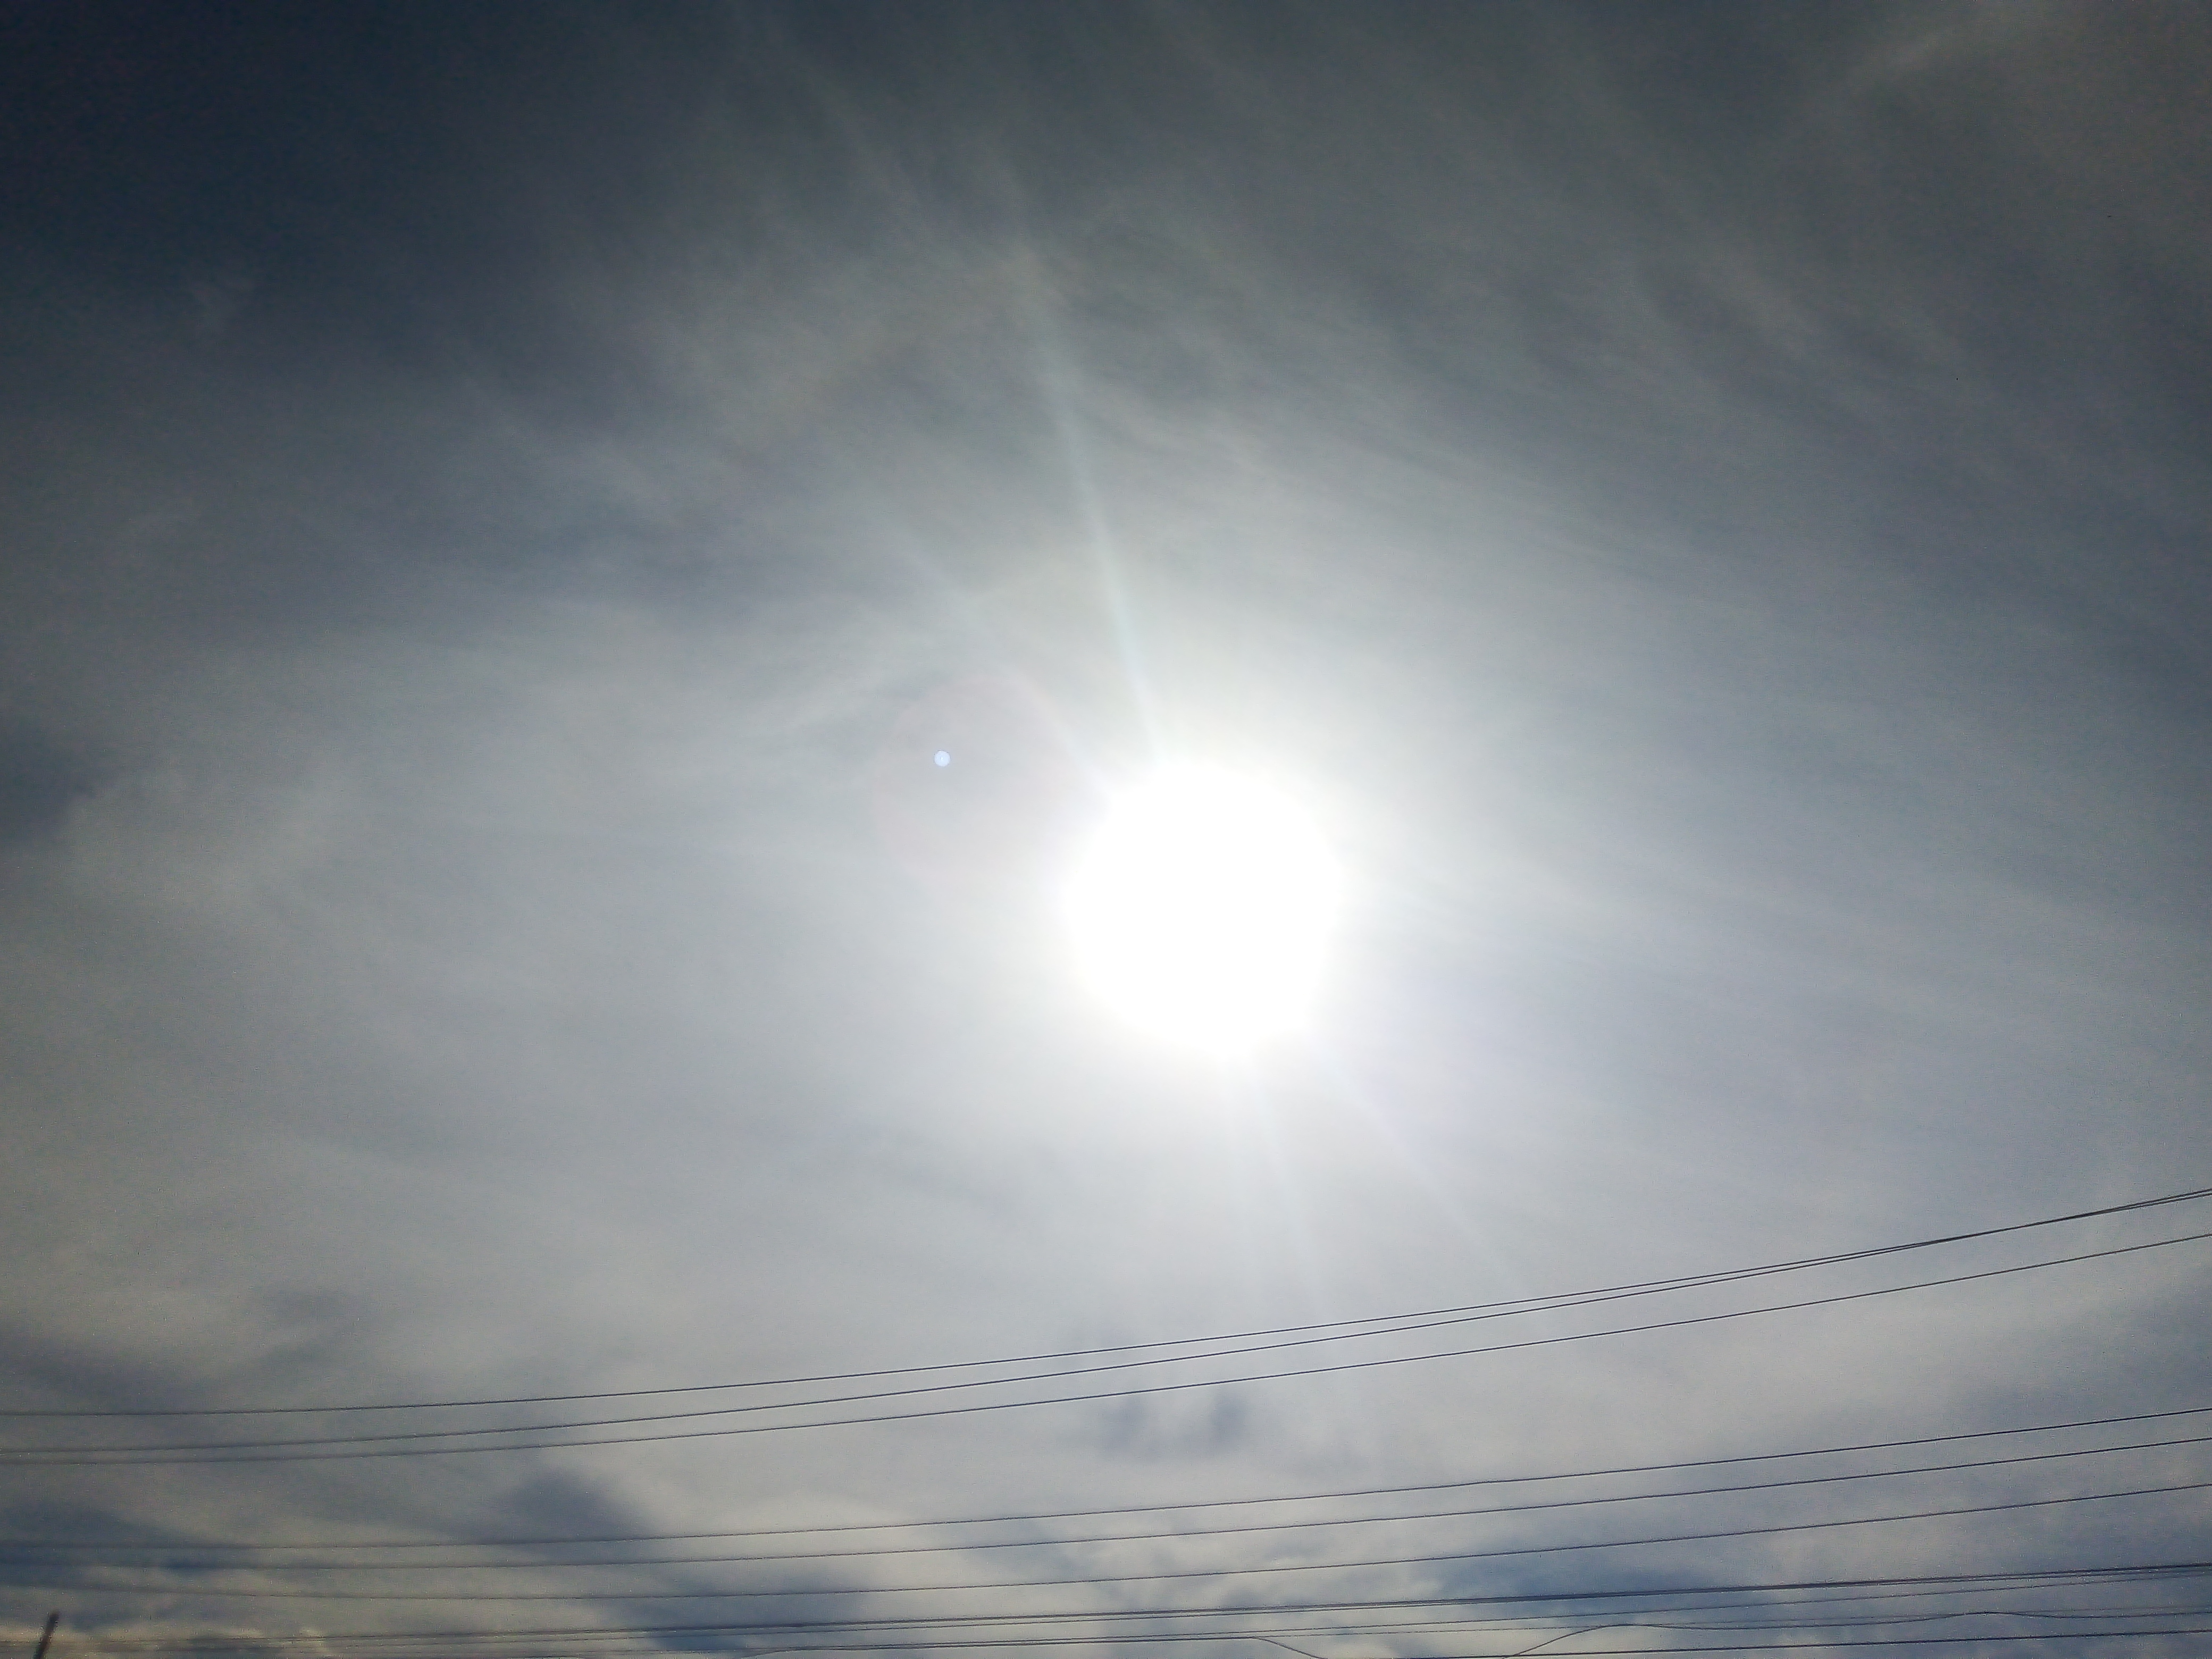
\includegraphics[width=0.9\textheight,keepaspectratio=true]{clouds/cirrostratus_fibratus}
    \caption{Перисто-слоистые, Cirrostratus fibratus}
    \label{fig:pp03}
    % https://commons.wikimedia.org/wiki/File:Sun_Halo_Salinas_Victoria_Desert.jpg
  \end{sidewaysfigure*}

  \begin{sidewaysfigure*}
    \centering
    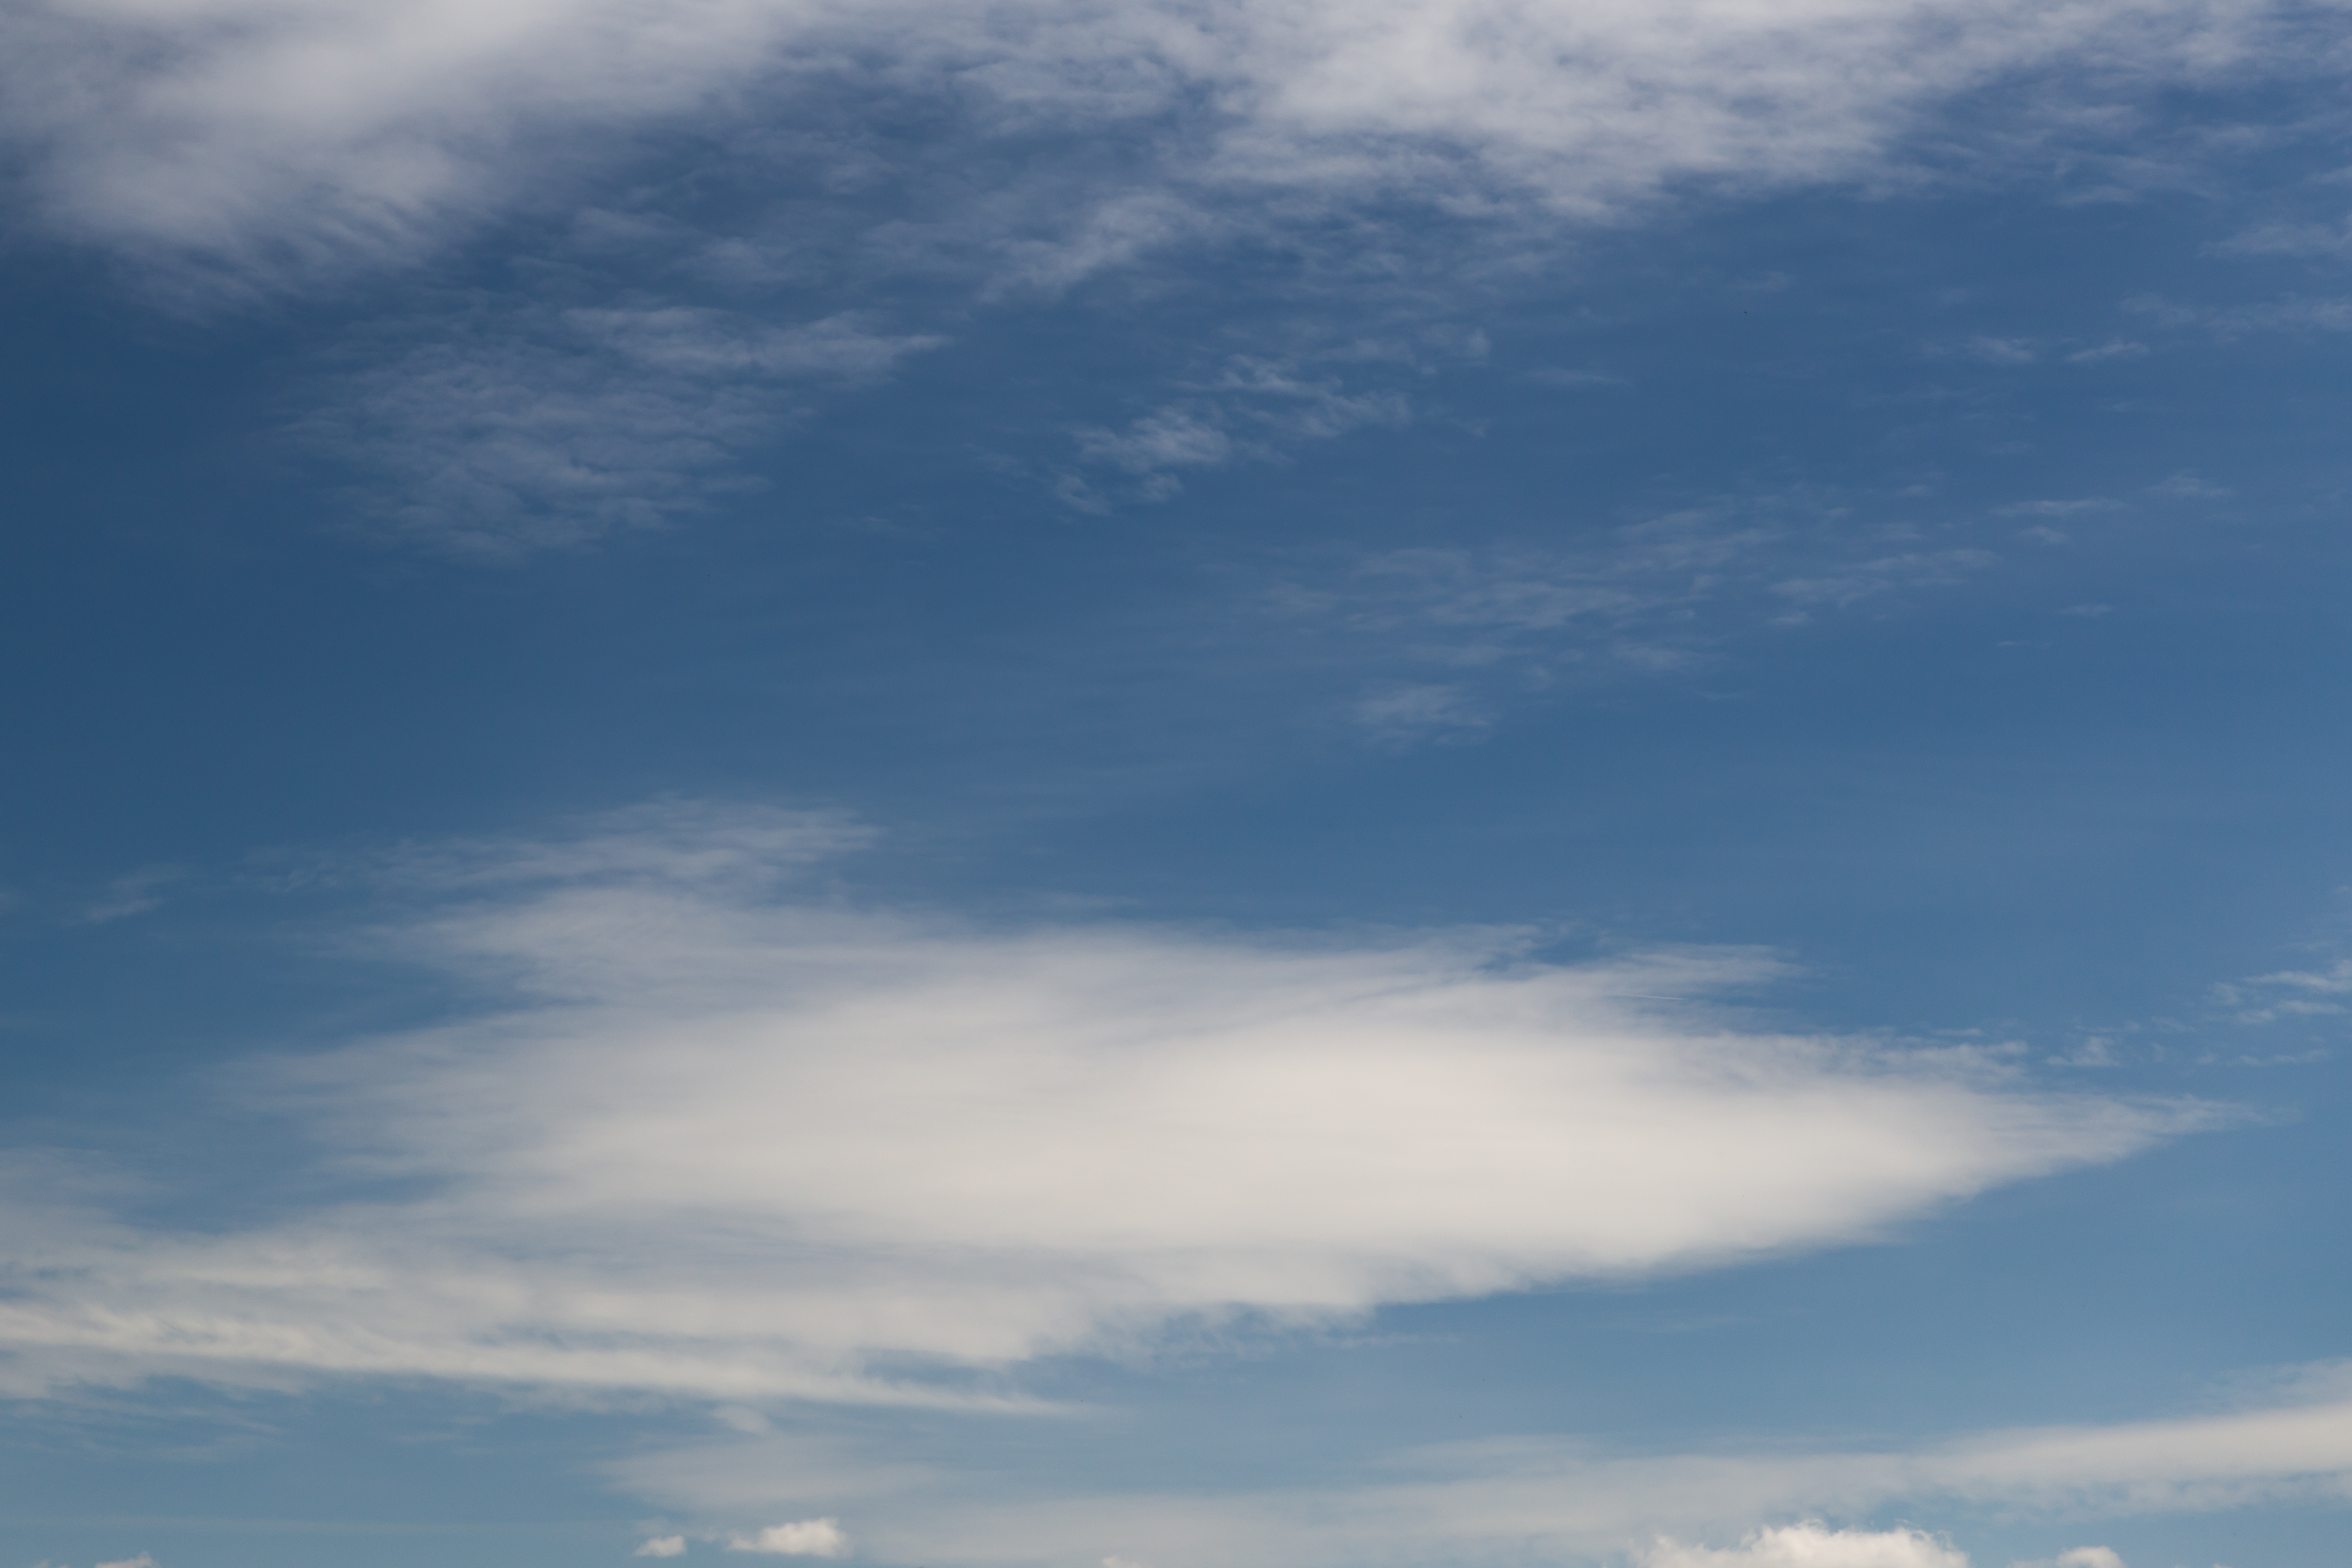
\includegraphics[width=0.9\textheight,keepaspectratio=true]{clouds/altocumulus_stratiformis}
    \caption{Altocumulus stratiformis}
    \label{fig:altocumulus-stratiformis}
    % https://commons.wikimedia.org/wiki/File:Altocumulus_stratiformis_-_20150430_12h46_(10127).jpg
  \end{sidewaysfigure*}

  \begin{sidewaysfigure*}
    \centering
    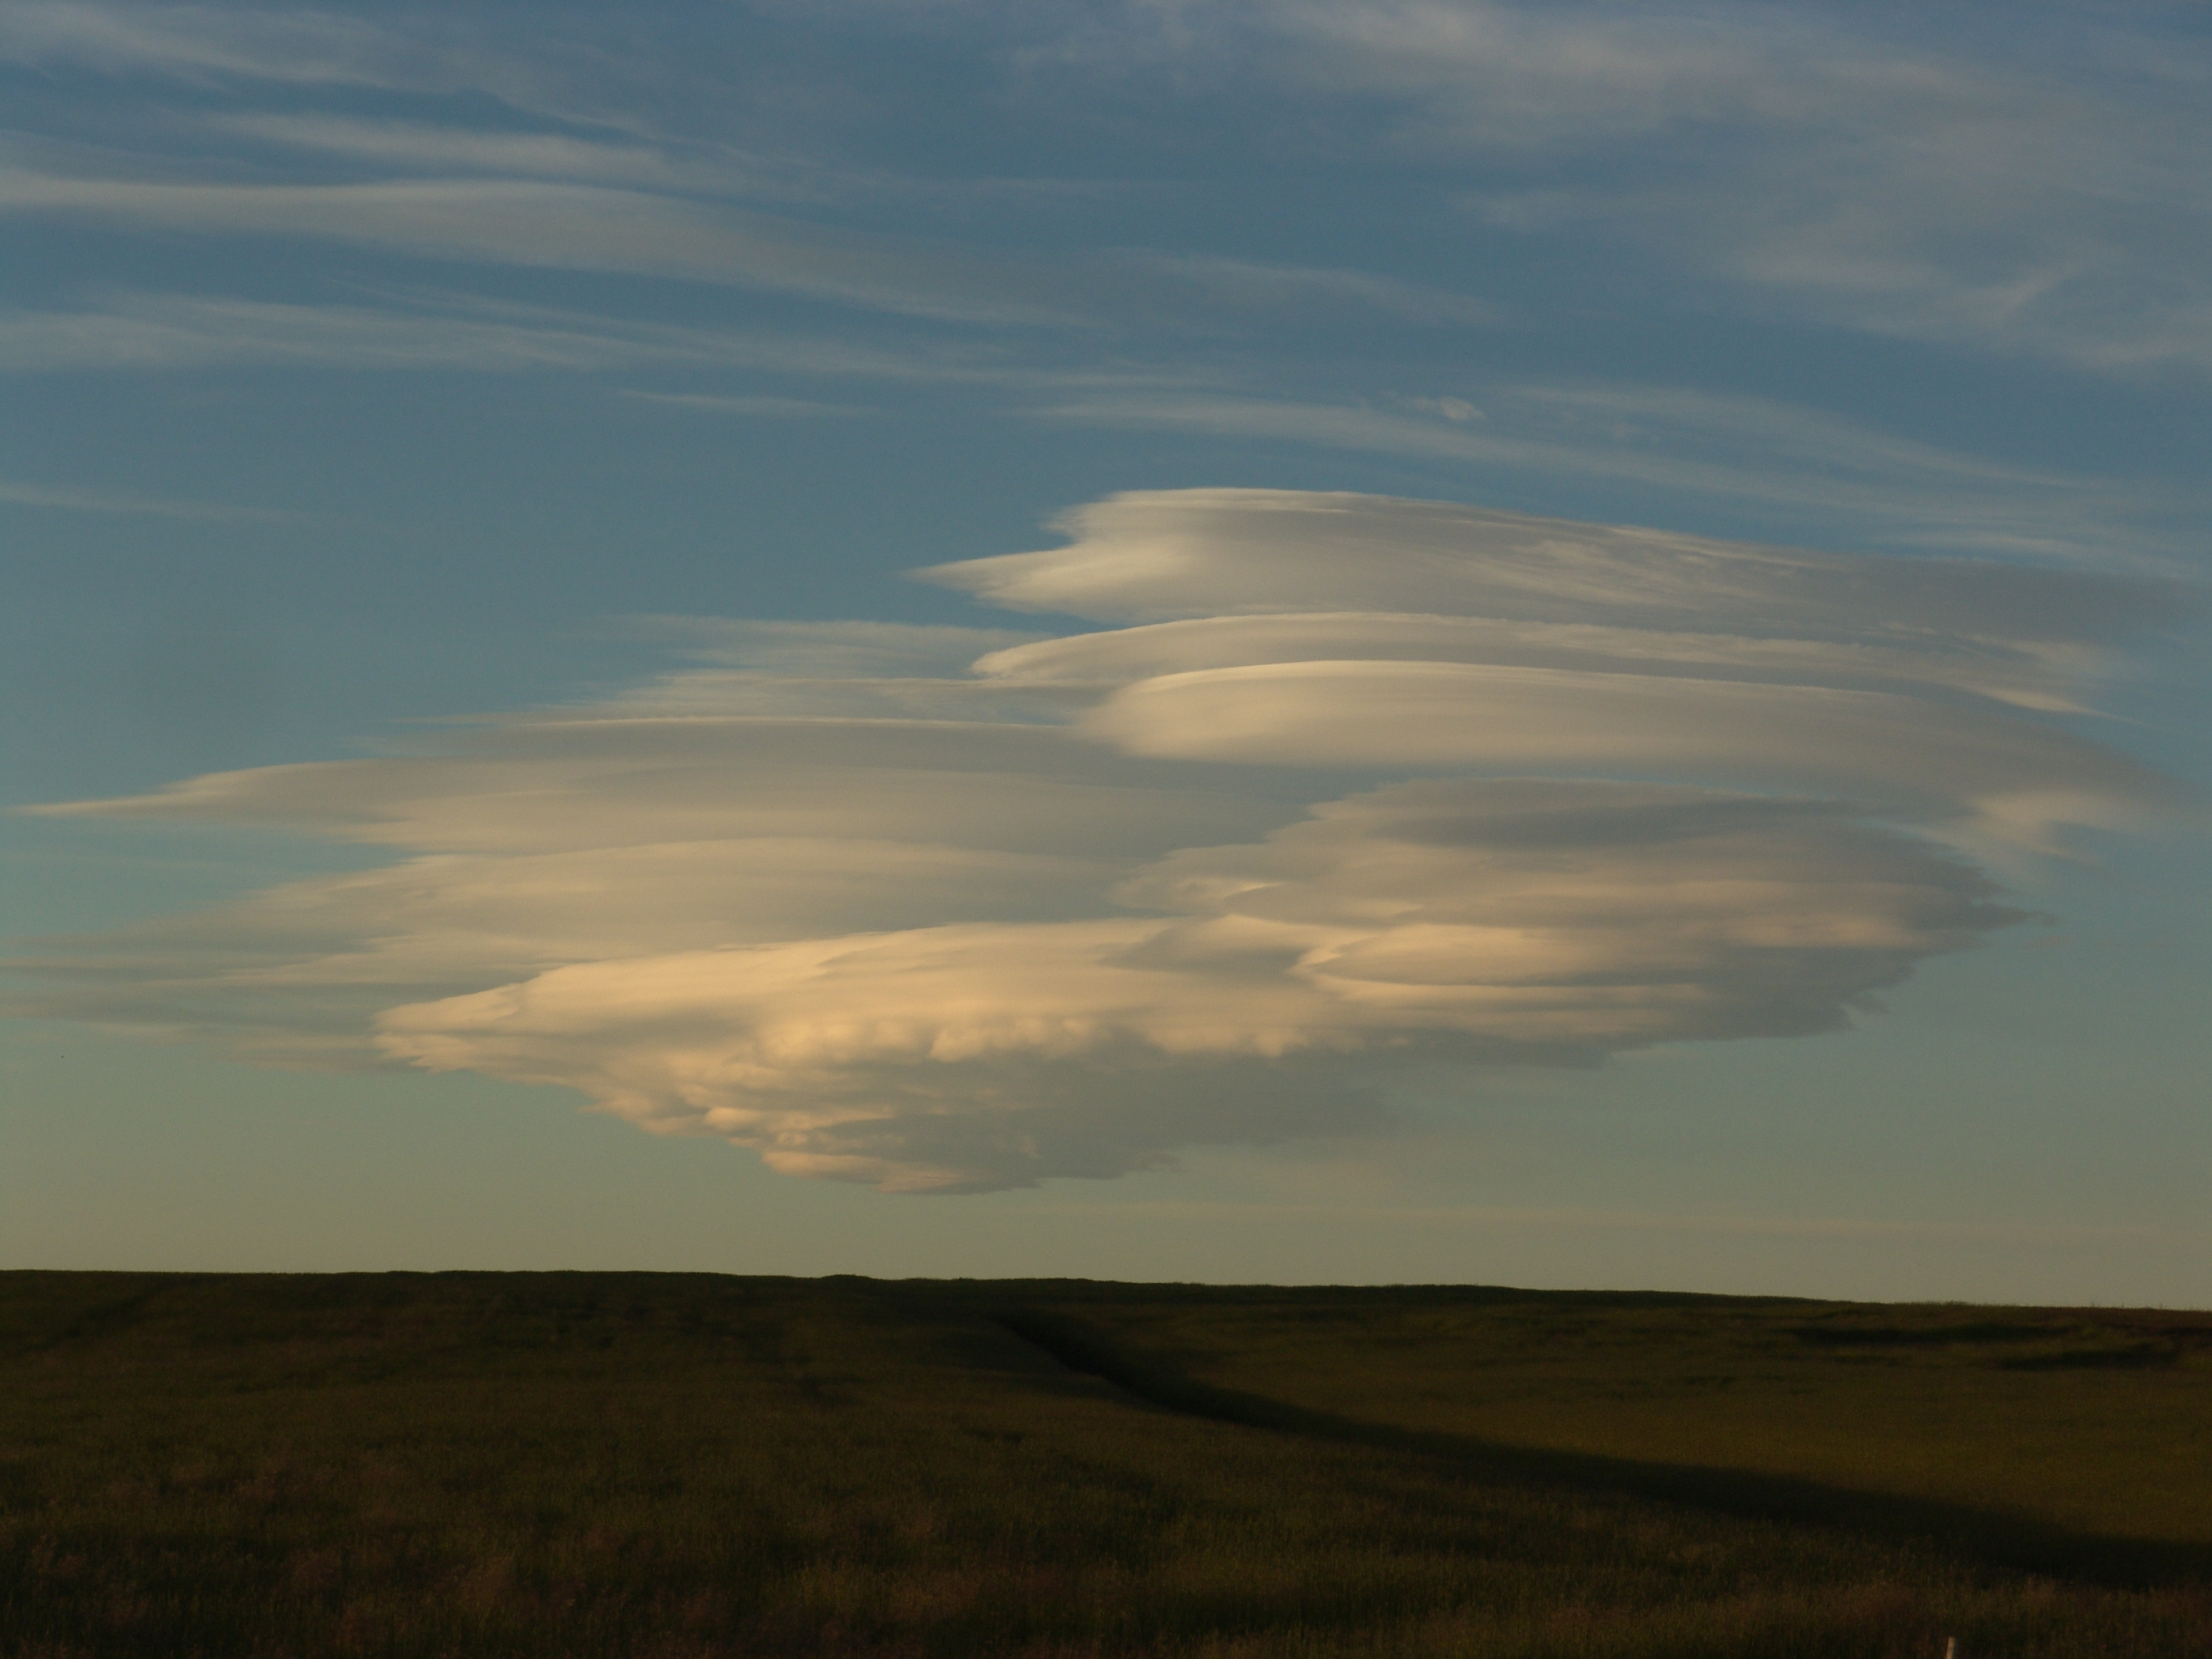
\includegraphics[width=0.9\textheight,keepaspectratio=true]{clouds/altocumulus_lenticularis}
    \caption{Altocumulus lenticularis}
    \label{fig:altocumulus-lenticularis}
    % https://commons.wikimedia.org/wiki/File:Iceland_Landscape_4453.JPG
  \end{sidewaysfigure*}

%%% Local Variables:
%%% mode: latex
%%% TeX-master: "yacht-captain"
%%% End:
